\subsection{Analysis of Distance Estimates}

\subsubsection{Model / Manual Distance Comparison}\label{subsubsec:distance_comparison}

In this section, the precision and accuracy of the distance estimates generated using the
four configurations of the distance estimation pipeline (outlined in
Section~\ref{subsubsec:configuratons}) are evaluated.
In order for these data to be analysed, the estimates are benchmarked against their
corresponding manual distance estimates (supplied with the dataset), thus these estimates
use detection frames originating from the manual sample (Section~\ref{subsubsec:sampling}).

Ideally, each and every manual distance should be joined to its corresponding modelled
distance estimate; however, due to the absence of any frame-position data associated
with the manual annotations, automating this using traditional algorithms is impossible
in circumstances where multiple chimps are captured in a single frame.
This is because when multiple individuals are detected, there is ambiguity in regard to
which distance a given modelled distance should be joined to.
Moreover, approaching this task manually is extremely labour-intensive and was therefore
outside the scope of this project.
As a result, this analysis focuses on distance comparisons associated with frames capturing
only a single individual.

Upon joining the modelled distance estimates to their corresponding manual estimates, the
overall errors of each of the four pipeline configurations were calculated.
Table~\ref{tab:overall_errors} shows the mean average error, root mean squared error,
average difference (i.e., mean($model_i$ - $manual_i$)) and the result of a statistical
difference test (i.e., where p-value < 0.05).
To note, while both the mean average and root mean squared errors give a measure of the
absolute error of the configurations, the average difference does not and is affected by
cancellation between overestimates and underestimates.
Therefore, it is used as a metric to assess whether a given configuration over or
under-predicts relative to the manual distance estimation method, where a positive value
indicates over-prediction while a negative value indicates under-prediction.

The modelled distance estimates were then grouped by their corresponding manual estimates (i.e.,
0.5 m, 1.0 m, \ldots 15 m).
Figure~\ref{fig:distance_comparison} shows the averages of the modelled estimates for each
group while Figure~\ref{fig:spread_comparison} shows each individual modelled estimate for
each group, giving a visualisation of the spread of the estimates.
Table~\ref{tab:regression_gradients} shows the gradients of the fitted regression lines
correlating the averages of all grouped distance estimates with their corresponding manual
distance estimate for each configuration.
These individual errors for each of these groups were then calculated.
Figure~\ref{fig:mae} show the change in mean average error for each group while
Figure~\ref{fig:rmse} shows the change in root mean squared error for each group.

\vspace{1cm}

\begin{table}[htbp]
    \centering
    \caption{Mean average error (MAE), root mean squared error (RMSE), average difference between
    model and manual estimate ($\Delta_{average}$) and result of Wilcoxon signed rank test for
    statistical difference. These data describe all distance estimates for each pipeline
    configuration collectivelly.)}
    \label{tab:overall_errors}
    \begin{tabular}{ccccc}
        \textbf{Method} & \textbf{MAE / m} & \textbf{RMSE / m} & \textbf{$\Delta_{average}$ / m}
        & \textbf{Statistical Difference} \\
        \midrule
        DPT, BBOX & 1.81 & 2.66 & 0.586 & YES \\
        DPT, SEG  & 1.70 & 2.45 & 0.836 & YES \\
        DA, BBOX  & 2.03 & 2.62 & 1.49  & YES \\
        DA, SEG   & 3.00 & 3.52 & 2.80  & YES \\
    \end{tabular}
\end{table}

\clearpage

\begin{figure}[H]
    \centering
    \vspace{1cm}
    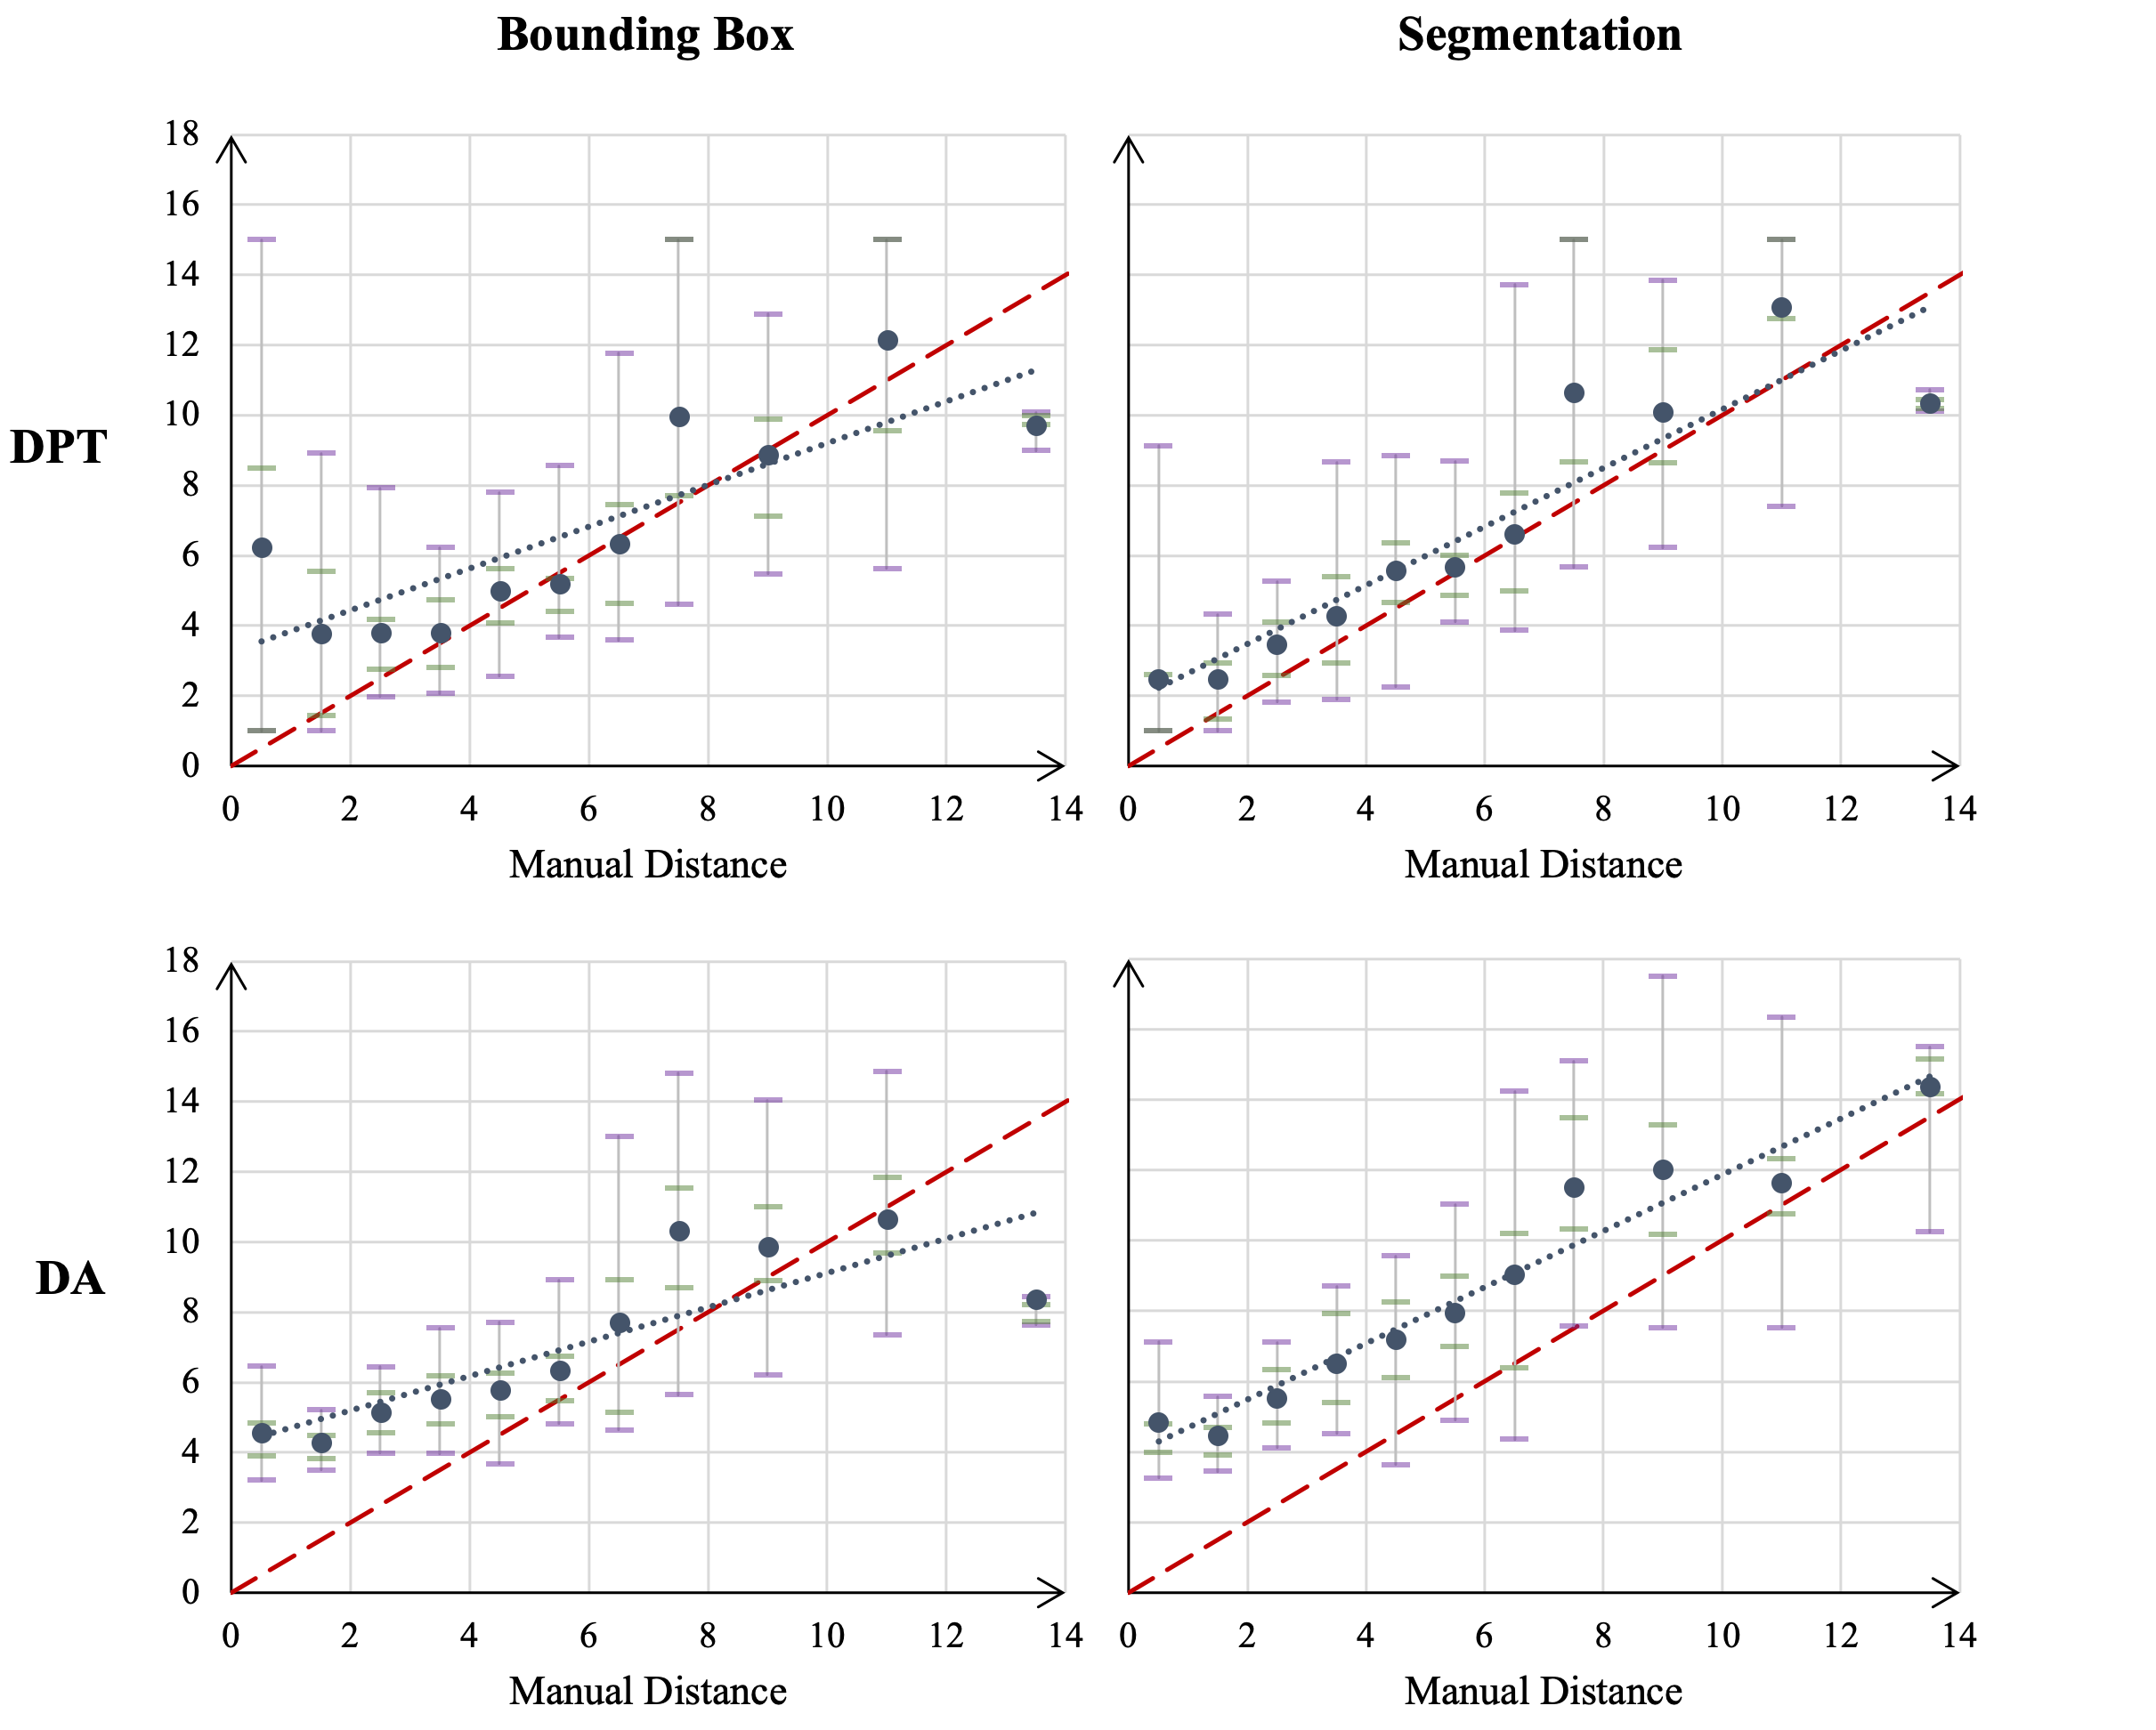
\includegraphics[width=1.01\textwidth]{body/analysis/assets/distance_graphs/averages}
    \caption{Graphs showing mean modelled distance estimates mapped to thier corresponding manual
    estimates for the configurations: DPT/bounding box (top-left), DPT/segmentation (top-right),
        DA/bounding box (bottom-left) and DA/segmentation (bottom-right). The blue dotted line
        shows the fitted regression line. The red dashed line shows the ideal (i.e., model=manual).
        the error bars show the 25–75 (green) and 5–95 (purple) percentiles. All distances are in
        units of meters.}
    \label{fig:distance_comparison}
\end{figure}

\vspace{1cm}

\begin{table}[H]
    \centering
    \caption{Gradients of the regression lines (blue dotted lines in Figure~\ref{fig:distance_comparison})
        correlating the averages of all binned distance estimates with their corresponding manual distance
        estimate for each configuration.}
    \label{tab:regression_gradients}
    \begin{tabular}{cc}
        \textbf{Method} & \textbf{Regression Gradient}\\
        \midrule
        DPT, BBOX & 0.59 \\
        DPT, SEG  & 0.84 \\
        DA, BBOX  & 0.49 \\
        DA, SEG   & 0.80 \\
    \end{tabular}
\end{table}

\begin{figure}[p]
    \centering
    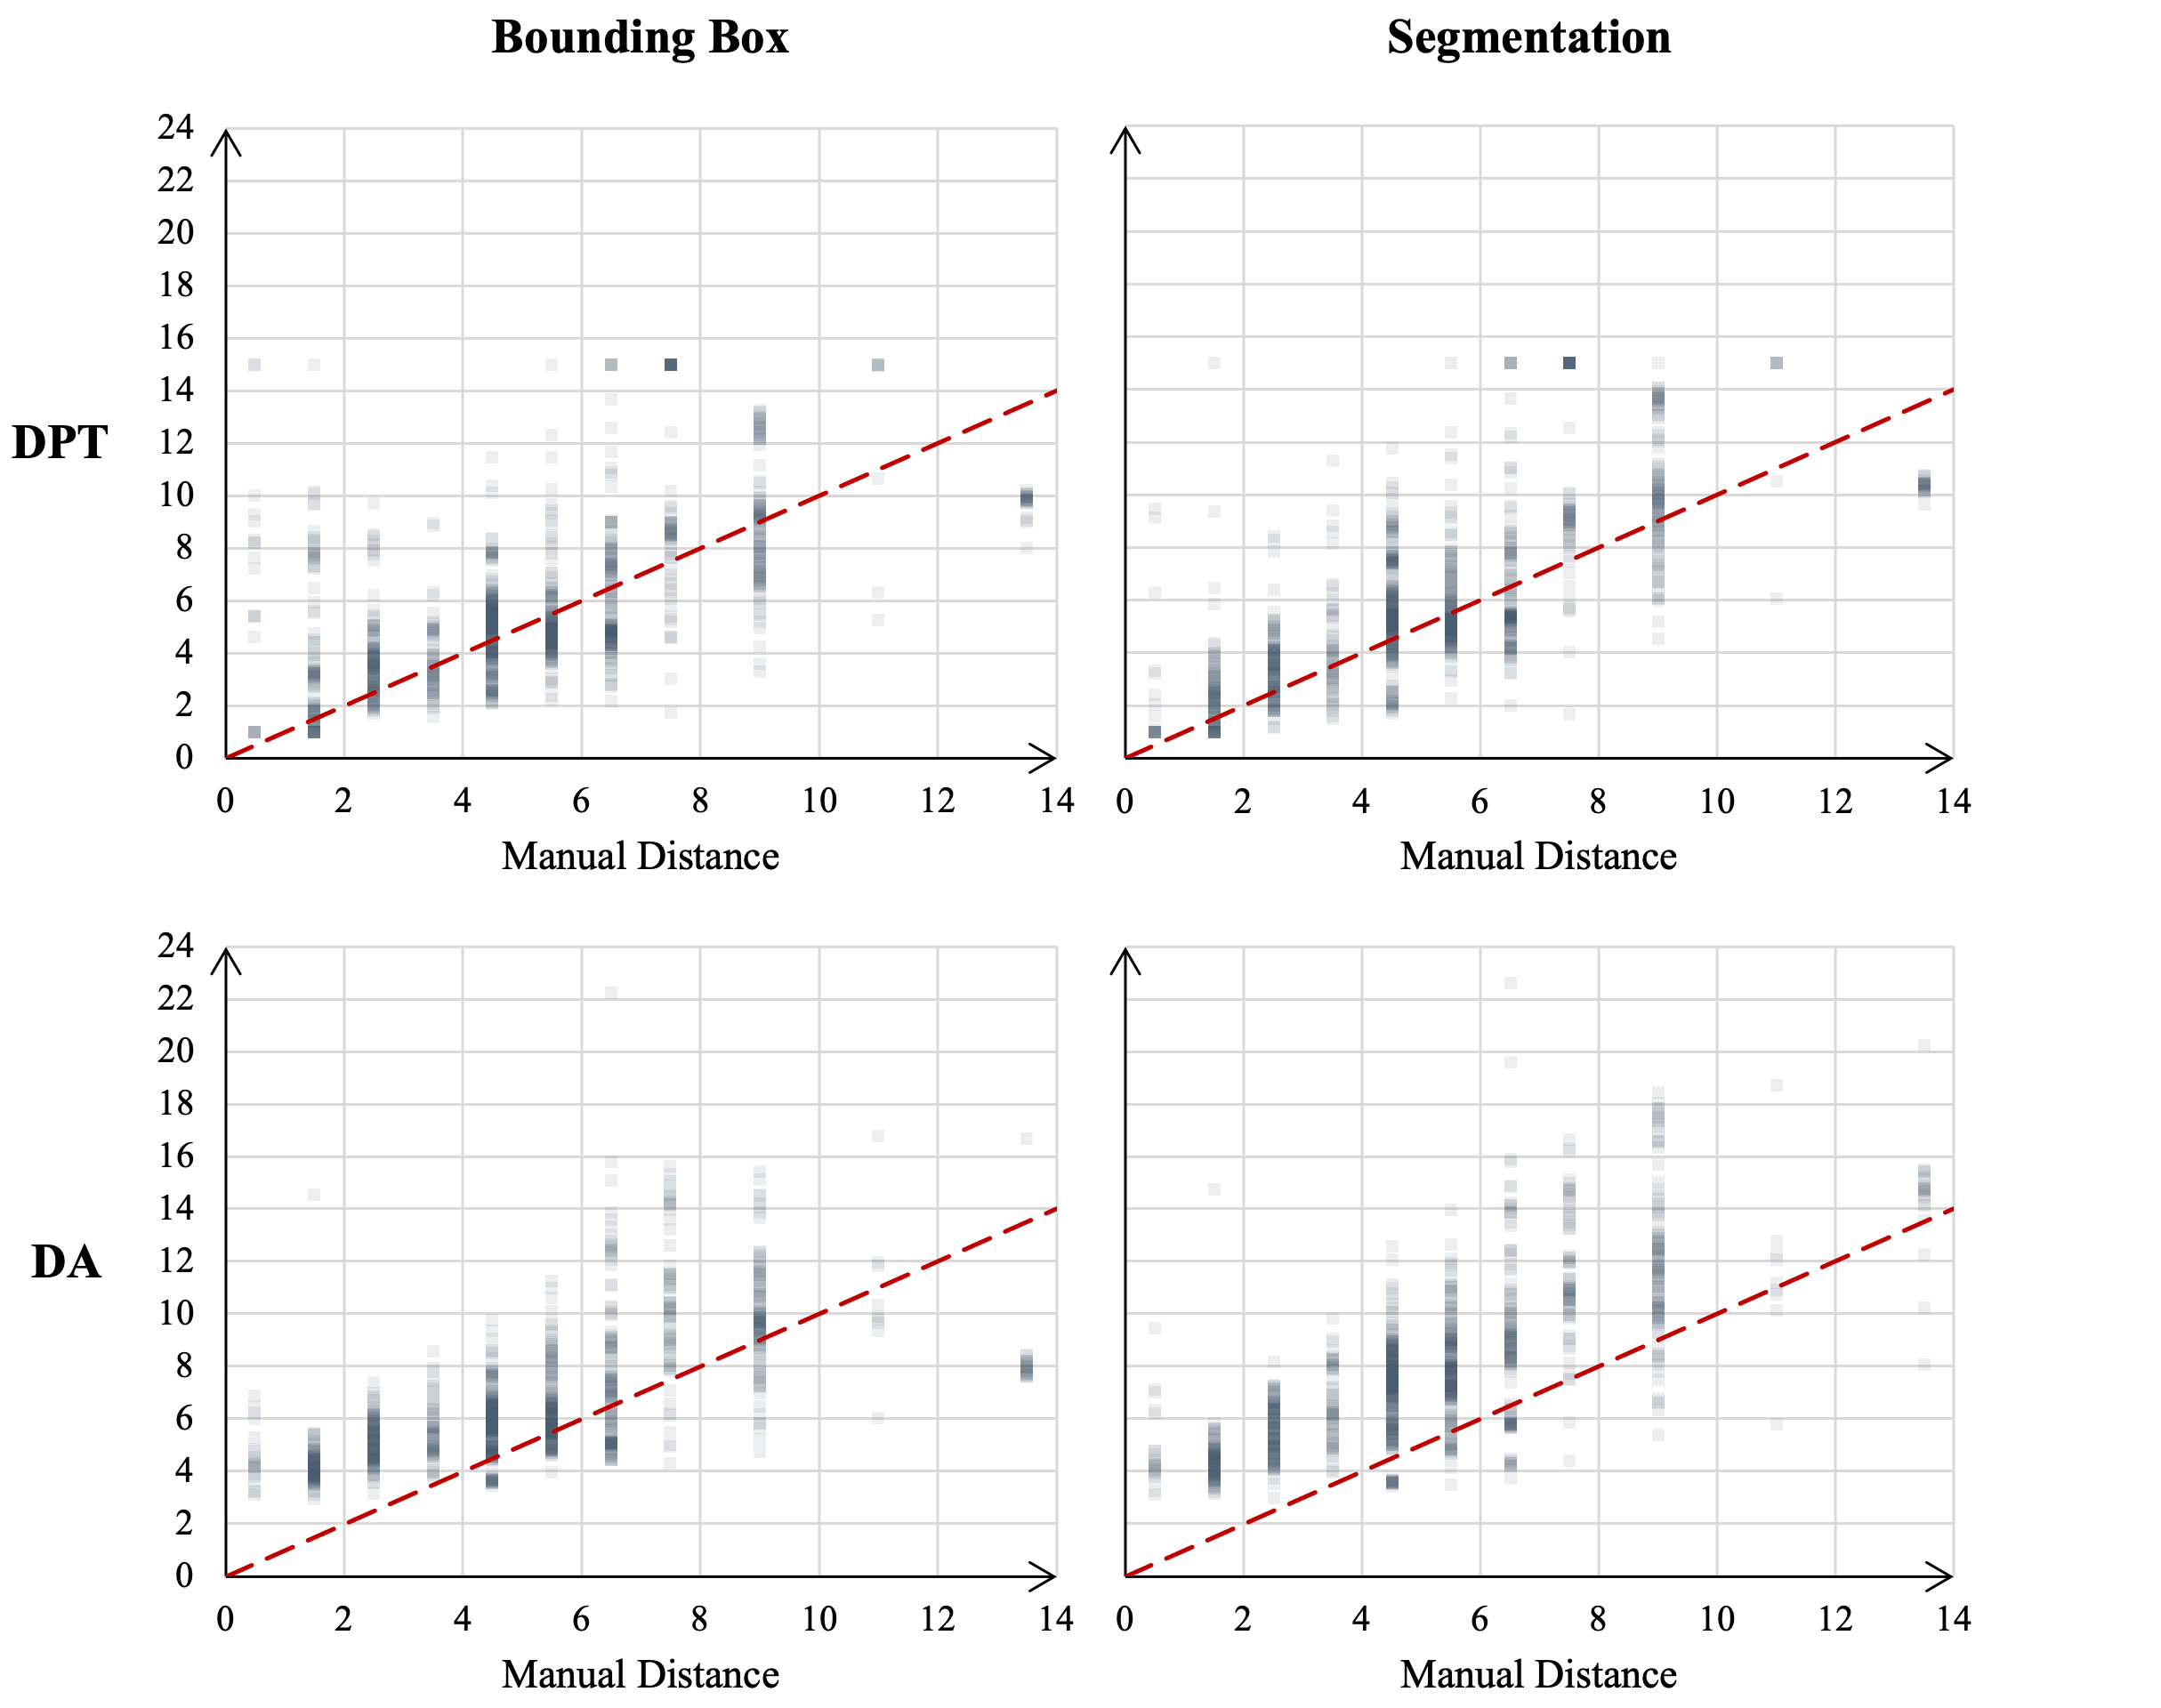
\includegraphics[width=1.01\textwidth]{body/analysis/assets/distance_graphs/spread}
    \caption{Graphs showing all modelled distance estimates mapped to thier corresponding manual
        estimates for the configurations: DPT/bounding box (top-left), DPT/segmentation (top-right),
        DA/bounding box (bottom-left) and DA/segmentation (bottom-right). The red dashed line shows
        the ideal (i.e., model=manual). All distances are in units of meters.}
    \label{fig:spread_comparison}
\end{figure}

\clearpage

\begin{figure}[H]
    \vspace{1cm}
    \centering
    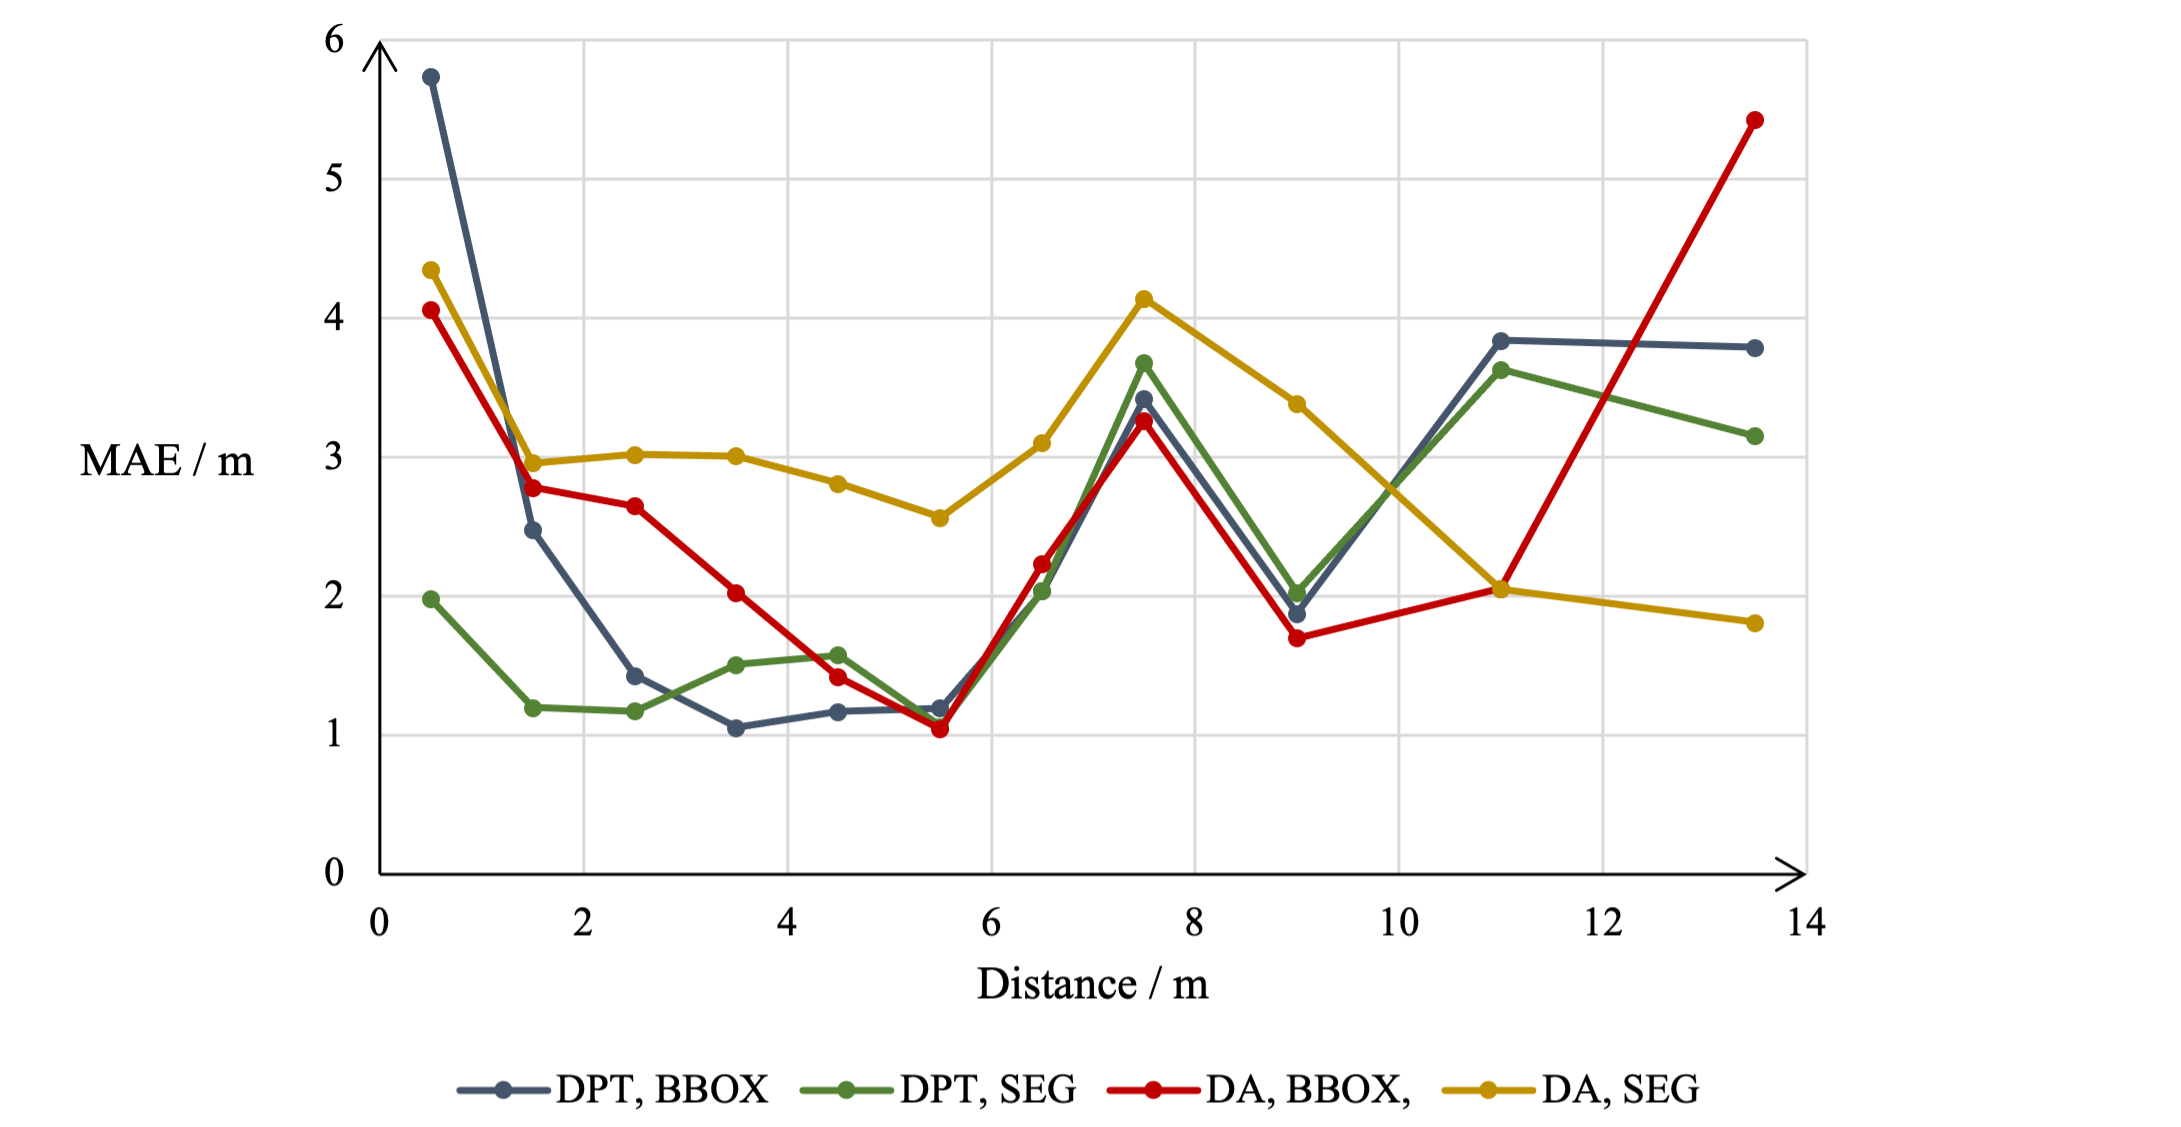
\includegraphics[width=1.01\textwidth]{body/analysis/assets/errors/MAE}
    \caption{Mean average error for distance estimates grouped by their corresponding manual
    estimates for each pipeline configuration.}
    \label{fig:mae}

    \vspace{2cm}

    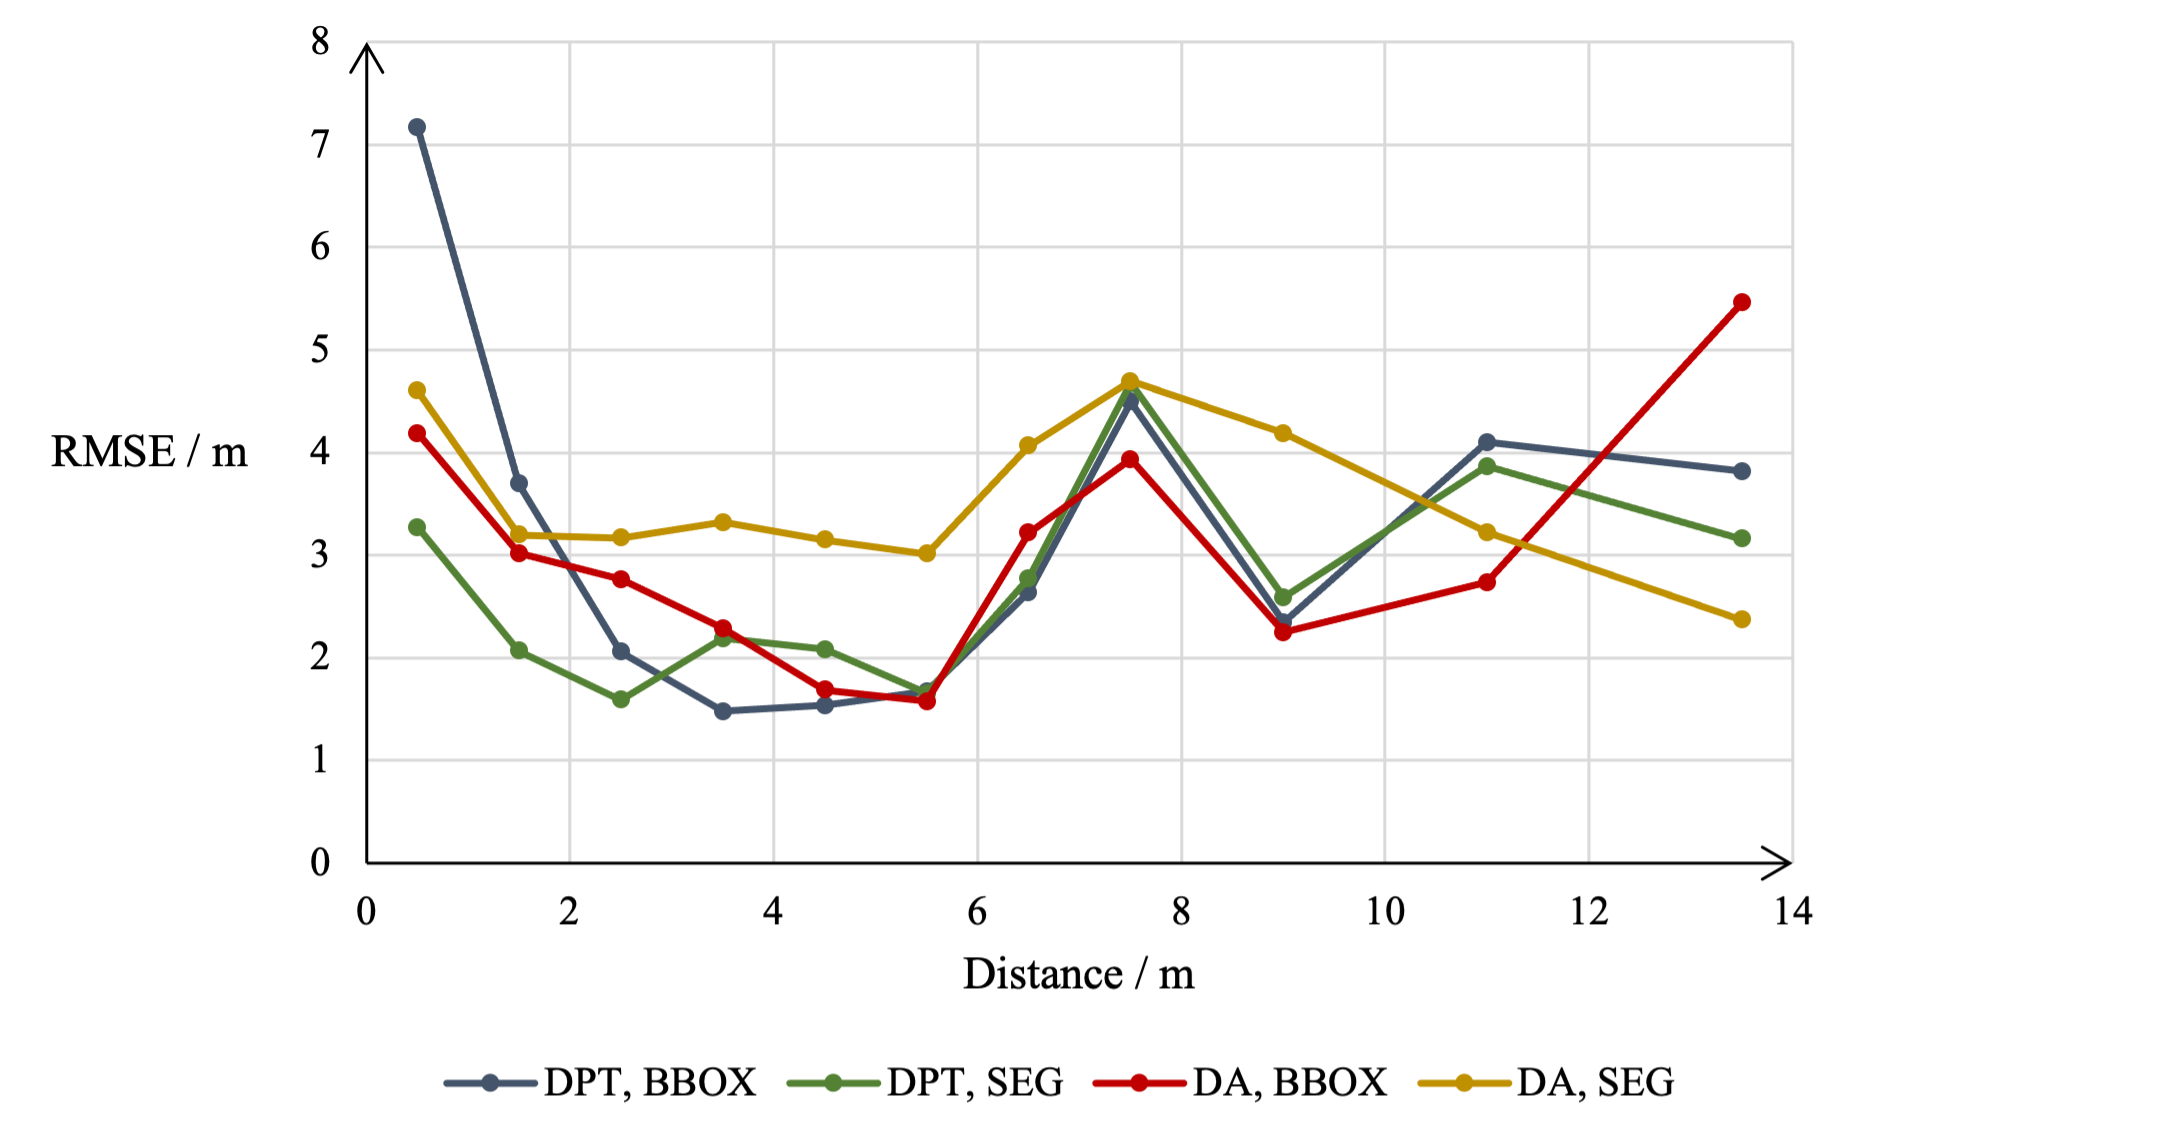
\includegraphics[width=1.01\textwidth]{body/analysis/assets/errors/RMSE}
    \caption{Root mean squared error for distance estimates grouped by their corresponding manual
    estimates for each pipeline configuration.}
    \label{fig:rmse}
\end{figure}

\clearpage

\textbf{Detection Method Effects}

Contrasting the distance estimates of the two detection method using DPT distance estimation,
an increase in both accuracy and precision is observed for the segmentation method compared
to the bounding box method at close distances (i.e., < 2 meters).
For modelled distances corresponding to manual estimates of 0.5 meters, the bounding box
method gives a MAE of 5.74 meters, a RMSE of 7.17 meters and an interquartile range of 7.50
meters while the segmentation method gives a MAE of 1.98 meters, a RMSE of 3.27 meters and
an interquartile range of 1.61 meters.
This is explained by a better detection frame calibration alignment.
Here, only the detection frame pixels defined by the chimpanzee segmentation are masked as
opposed to those within the entire bounding box.
As a result, more pixels corresponding to the transect background which are common to both
the calibration and detection frames are available for depth scale alignment, leading to a
superior calibration of the detection frame depth scale.

This effect is exemplified in Figure~\ref{fig:bbox_vs_seg_close_dpt}, where the bounding box
method results in an effectively failed calibration while the segmentation method succeeds.

\begin{figure}[htbp]
    \centering
    \makebox[0.8\textwidth][c]{
        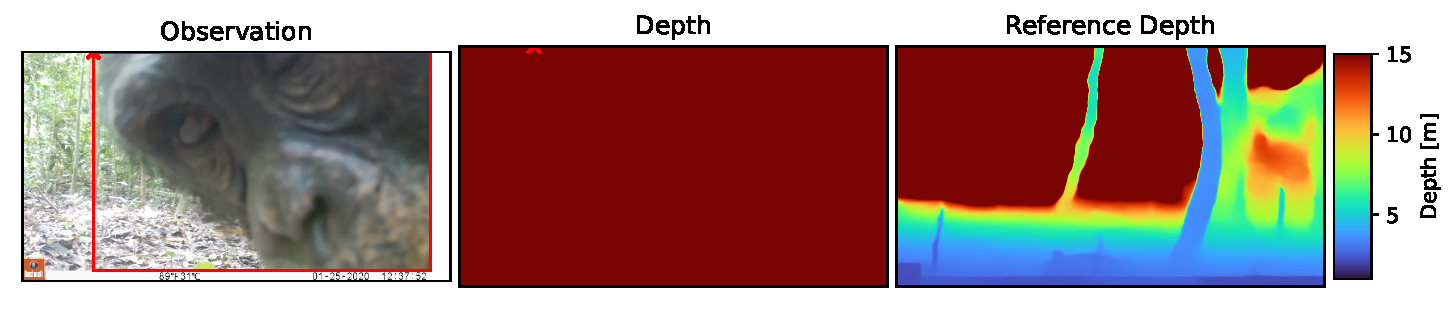
\includegraphics[width=0.9\textwidth]{body/analysis/assets/depth_maps/close_bbox_dpt}
    }\\[1mm]
    \makebox[0.8\textwidth][c]{
        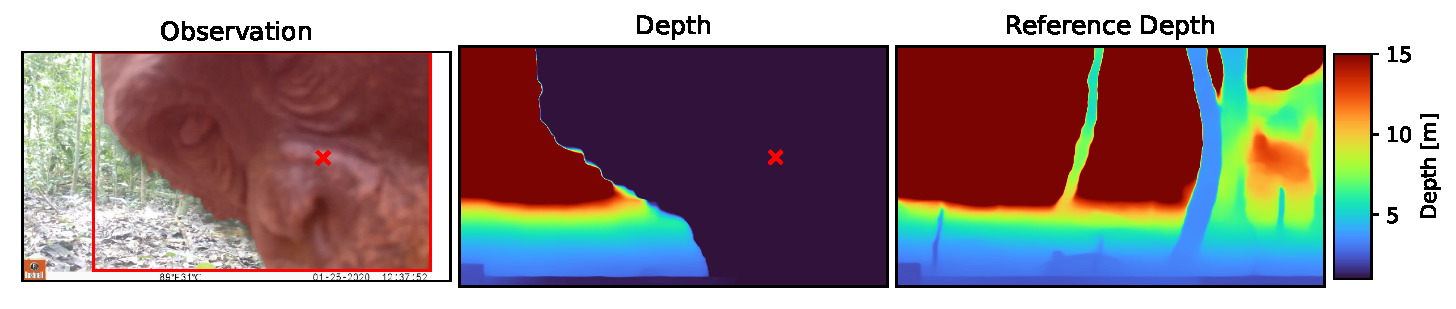
\includegraphics[width=0.9\textwidth]{body/analysis/assets/depth_maps/close_seg_dpt}
    }
    \caption{Example of DPT depth maps generated using bounding box (top) and segmentation
        (bottom) detection methods at a detection distance of 0.5 meters (manual estimate).
        In this example, the bounding box method gives a distance estimate of 15.0 meters
        while the segmentation method gives a distance estimate of 1.0 meters}
    \label{fig:bbox_vs_seg_close_dpt}
\end{figure}

In contrast, this detection effect does not apply when Depth Anything is used to estimate
distance.
No significant difference is observed in the accuracy and/or precision of the distance
estimates obtained using the two detection methods.
For modelled distances corresponding to manual estimates of 0.5 meters, the bounding box
method gives a MAE of 4.06 meters, a RMSE of 4.19 meters and an interquartile range of 0.95
meters while the segmentation method gives a MAE of 4.35 meters, a RMSE of 4.60 meters and
an interquartile range of 0.80 meters.
This is an expected result given that Depth Anything is a metric depth model.
Unlike with DPT, the scale of the generated depth maps are not aligned to that of the reference
frames meaning that the detection method does not influence this scale.
Therefore, it can be inferred that the difference in distance estimates given by these detection
methods is a result of the different pixel sampling techniques used to calculate the final distance
estimate (i.e., bounding box depth from the pixel corresponding to the 20th percentile depth
and segmentation depth from the depth of the centre-most pixel) rather than differences on depth
scaling.

Figure~\ref{fig:bbox_vs_seg_close_da} shows the corresponding Depth Anything depth maps using both
detection methods for the same example shown in Figure~\ref{fig:bbox_vs_seg_close_dpt}.
It can be seen that both detection methods lead to identical depth maps, with the final detection
distance estimates being very close.

\begin{figure}[htbp]
    \centering
    \makebox[0.8\textwidth][c]{
        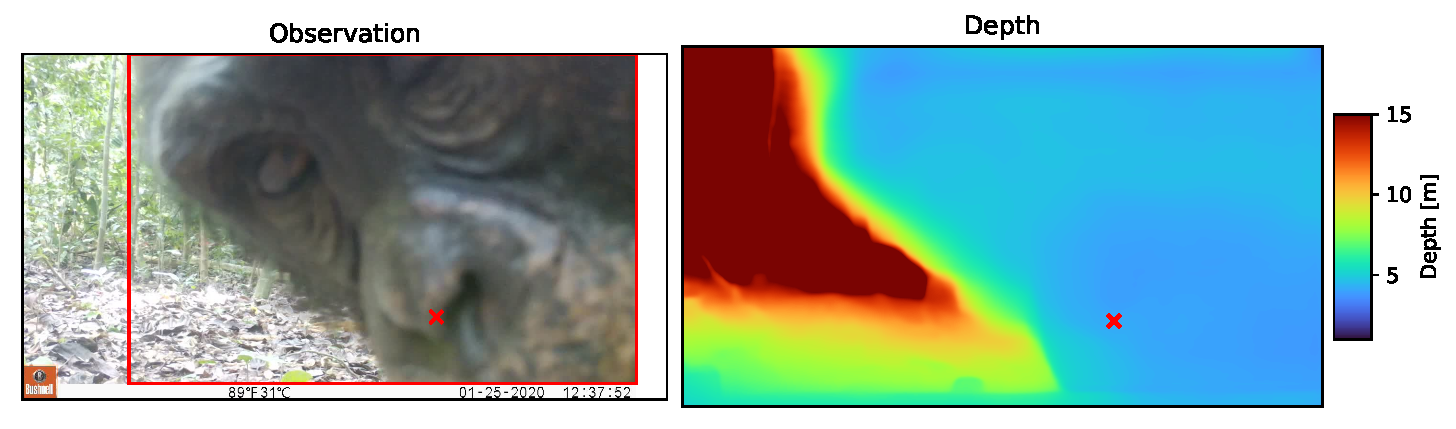
\includegraphics[width=0.7\textwidth]{body/analysis/assets/depth_maps/close_bbox_da}
    }\\[1mm]
    \makebox[0.8\textwidth][c]{
        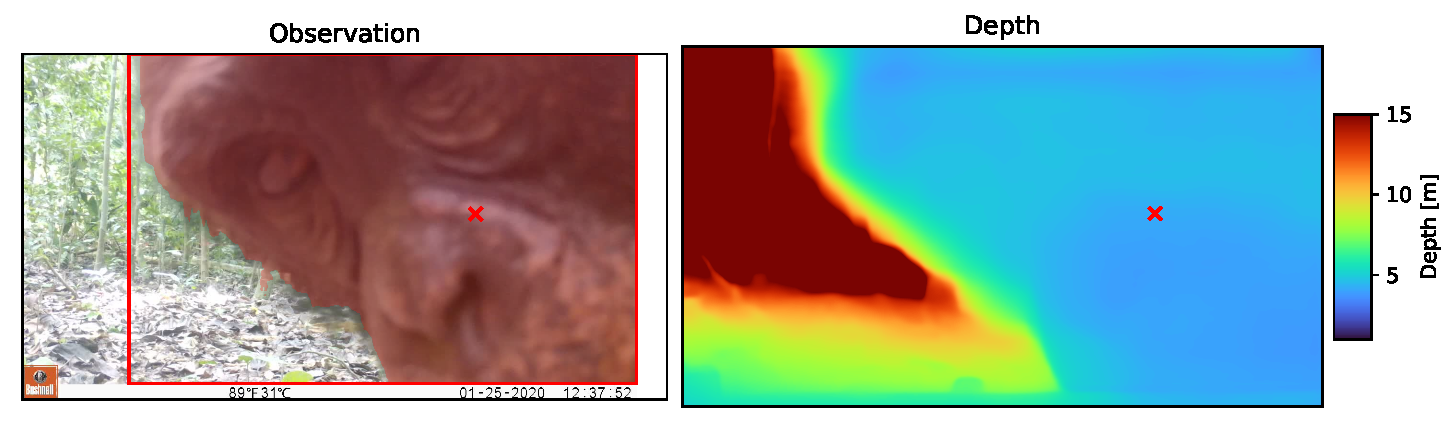
\includegraphics[width=0.7\textwidth]{body/analysis/assets/depth_maps/close_seg_da}
    }
    \caption{Example of Depth Anything depth maps generated using bounding box (top) and segmentation
        (bottom) detection methods at a detection distance of 0.5 meters (manual estimate).
        In this example, the bounding box method gives a distance estimate of 4.11 meters
        while the segmentation method gives a distance estimate of 4.17 meters.}
    \label{fig:bbox_vs_seg_close_da}
\end{figure}

Upon inspection of Table~\ref{tab:regression_gradients}, it can be seen that for both DPT and Depth
Anything models, the gradients of the regression lines (correlating the averages of the binned
distance estimates with the corresponding manual estimates) of the segmentation detection methods
are higher relative to their corresponding bounding box regression gradient and also better
correlated to the ideal.
A possible explanation for this trend is a minimised contribution of occluding pixels during the
final detection distance calculation at medium to long distances when using the segmentation method.
With this particular dataset, it is from these medium distances where detections start to become
occluded by foliage.
When the bounding box method is used, the final distance can be biased towards a lower estimate in
circumstances where a significantly large portion of the bounding box is composed of occluding pixels
that correspond to a significantly shorter distance.
Conversely, a high quality segmentation often avoids this.
This effect is exemplified in Figure~\ref{fig:bbox_vs_seg_occluded}.

\begin{figure}[htbp]
    \centering
    \makebox[0.8\textwidth][c]{
        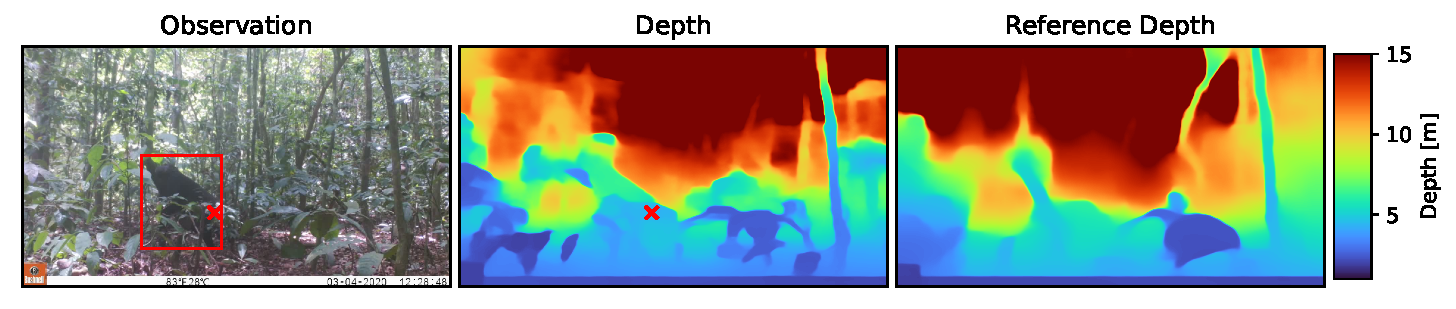
\includegraphics[width=0.9\textwidth]{body/analysis/assets/depth_maps/occluded_bbox}
    }\\[1mm]
    \makebox[0.8\textwidth][c]{
        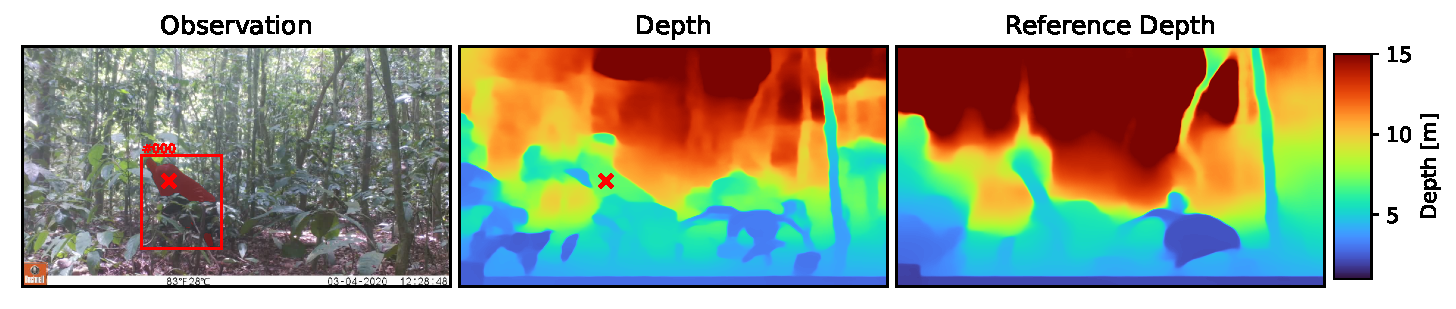
\includegraphics[width=0.9\textwidth]{body/analysis/assets/depth_maps/occluded_seg}
    }
    \caption{Example of DPT depth maps generated using bounding box (top) and segmentation
        (bottom) detection methods at a detection distance of 6.5 meters (manual estimate)
        where the detected individual is partially occluded by foliage. Here, the bounding
        box method gave a distance estimate of 4.40 meters while the segmentation method
        gave a distance estimate of 6.96 meters.}
    \label{fig:bbox_vs_seg_occluded}
\end{figure}

If, however, the quality of the segmentation is poor, the distances of occluded detections
may still be underestimated.
Figure~\ref{fig:haze_occluded} highlights a scenario where an individual was correctly detected
but, due to poor detection frame quality, the occluding foliage was instead segmented rather
than the individual.

\begin{figure}[htbp]
    \centering
    \makebox[0.8\textwidth][c]{
        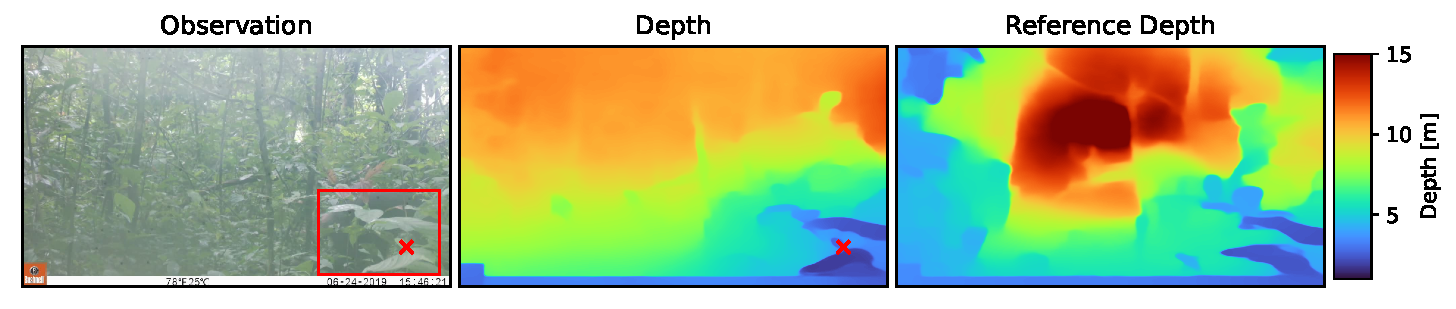
\includegraphics[width=0.9\textwidth]{body/analysis/assets/depth_maps/occluded_haze_bbox}
    }\\[1mm]
    \makebox[0.8\textwidth][c]{
        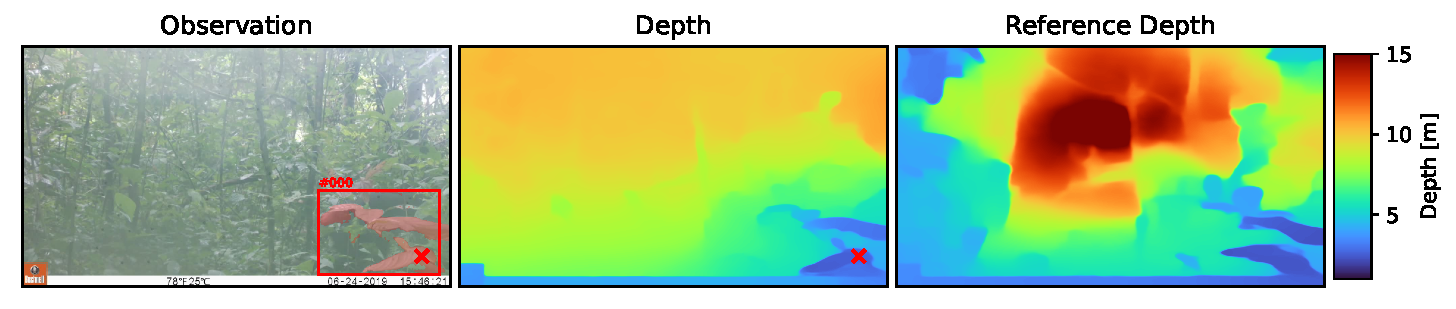
\includegraphics[width=0.9\textwidth]{body/analysis/assets/depth_maps/occluded_haze_seg}
    }
    \caption{Example of DPT depth maps generated using bounding box (top) and segmentation
        (bottom) detection methods at a detection distance of 4.5 meters (manual estimate)
        where the detected individual is partially occluded by foliage. Here, moisture on the
        camera lense has resulted in a slightly hazy image, leading to a failed segmentation
        of the detected individual. The bounding box method gave an estimated distance of
        2.64 meters while the segmentation method gave a distance estimate of 2.56 meters.}
    \label{fig:haze_occluded}
\end{figure}


Blurry detections frames

djou09

\vspace{5mm}
\textbf{Depth Model Effects}

As seen in Table~\ref{tab:regression_gradients}, the gradients of the regression lines
correlating the averages of the binned DPT distance estimates with respect to their manual
estimates are greater and also closer the ideal (gradient = 1) than that of Depth Anything.
This shows that, overall, DPT is better capturing the true scale of depth in the detection
frames than Depth Anything.
At short to medium distances (i.e., 2–7 meters), Figure~\ref{fig:distance_comparison} shows
that distance estimate averages closely follow a linear relationship, indicating that within
this distance region, both depth models are differentiating relative depth well.
However, Depth Anything generally over-predicts estimated depth in this region while the DPT
estimates are much closer to the ideal.
This trend also holds for the extreme-close distance region for Depth Anything (with both
detection methods) and also DPT using segmentation (DPT with bounding box over-predicts as
previously discussed).

While DPT gives a better measure of depth scale at close distances, the depth maps show that
Depth Anything is superior at differentiating the depth of fine-detail in the detection frames.
This is shown in Figure~\ref{fig:fine_detail}, where the depth maps generated by all
configurations with a common detection frame are shown side-by-side.


\begin{figure}[H]
    \centering
    \makebox[0.8\textwidth][c]{
        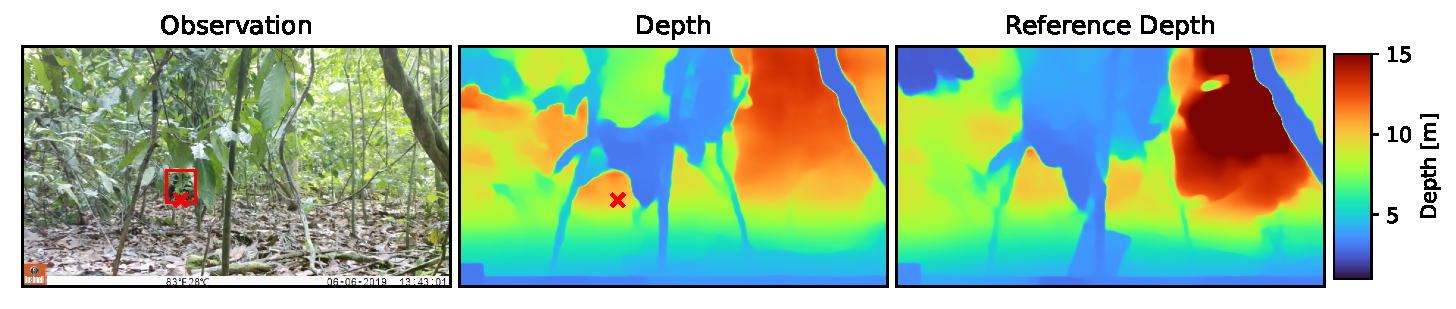
\includegraphics[width=0.9\textwidth]{body/analysis/assets/depth_maps/fine_detail/bbox_dpt}
    }\\[1mm]
    \makebox[0.8\textwidth][c]{
        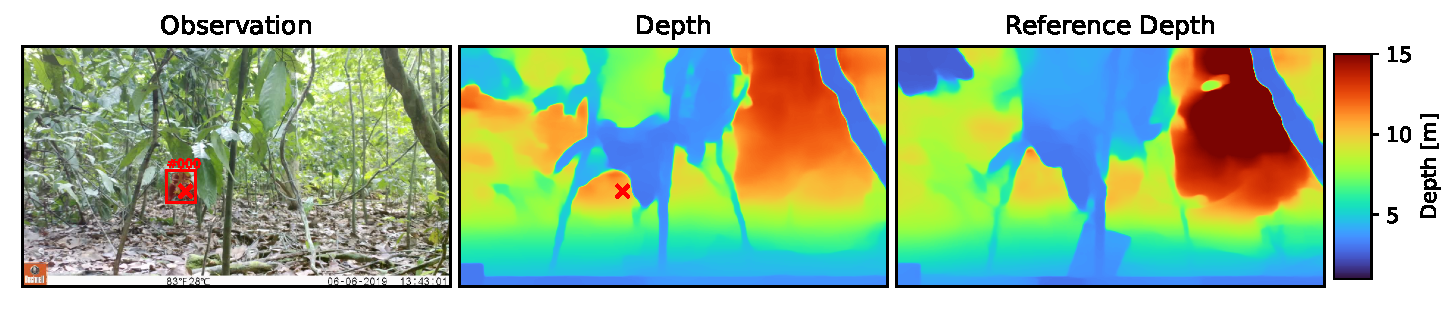
\includegraphics[width=0.9\textwidth]{body/analysis/assets/depth_maps/fine_detail/seg_dpt}
    }\\[1mm]
    \makebox[0.8\textwidth][c]{
        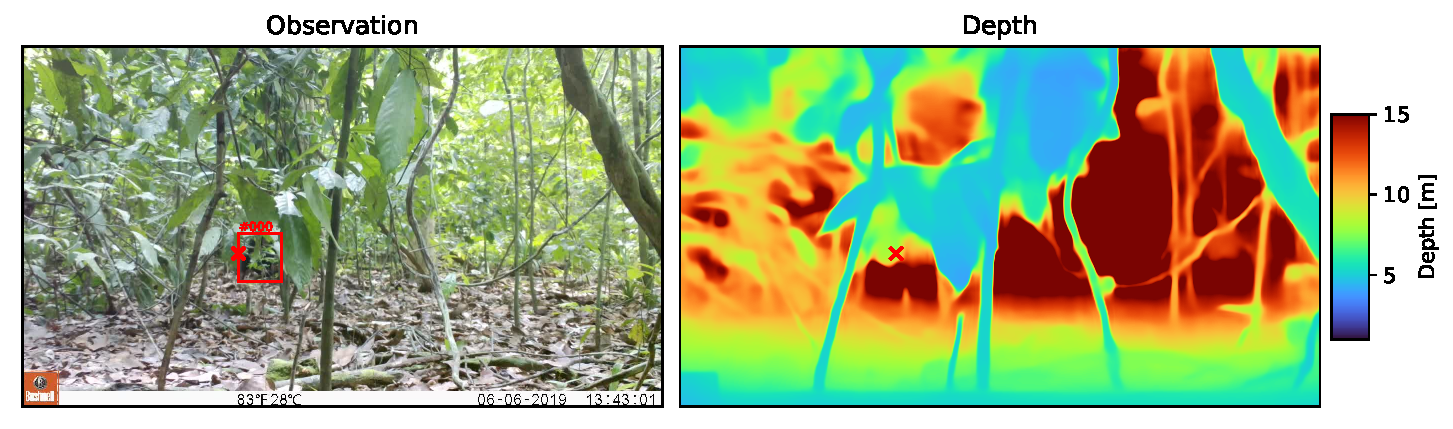
\includegraphics[width=0.7\textwidth]{body/analysis/assets/depth_maps/fine_detail/bbox_da}
    }\\[1mm]
    \makebox[0.8\textwidth][c]{
        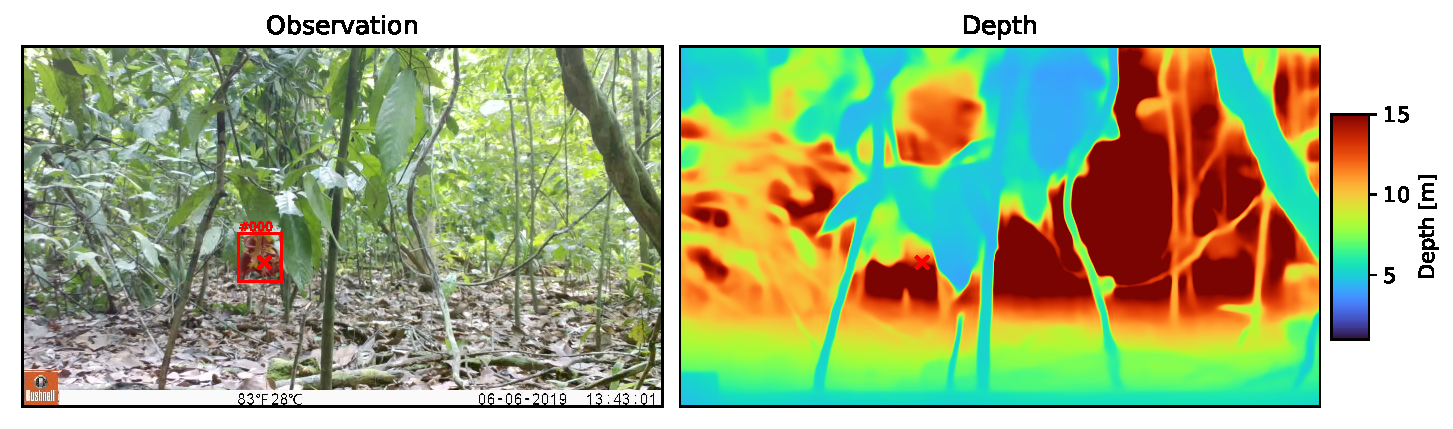
\includegraphics[width=0.7\textwidth]{body/analysis/assets/depth_maps/fine_detail/seg_da}
    }
    \caption{Example of depth maps generated using DPT/BBOX (row one), DPT/SEG
        (row two), DA/BBOX (row three) and DA/SEG (row four) detection methods at a detection
        distance of 13.5 meters (manual estimate). The following distance estimates were given:
        DPT/BBOX = 10.0 meters, DPT/SEG = 10.4 meters, DA/BBOX = 7.83 meters, DA/SEG = 13.6 meters.}
    \label{fig:fine_detail}
\end{figure}

The graphs in Figures~\ref{fig:distance_comparison} and~\ref{fig:spread_comparison} show that
for both DPT configurations as well as Depth Anything with bounding box, distance estimates
corresponding to manual estimates of 13.5 meters are significantly under-predicted.
This is not the case, however, for estimates given by Depth Anything using segmentation detection.
This is an interesting effect which is perfectly illustrated in Figure~\ref{fig:fine_detail}.
In this example both of the DPT depth maps fail to capture any significant differentiation in
depth within the small detection region.
As a result, the final distance estimates yield roughly equal values of approximately 10 meters.
In contrast, the Depth Anything depth map (identical for both detection methods) captures
much more detail in this region, therefore enabling the different pixel sampling techniques used
in the detection distance calculation to yield different results.
In the case of the bounding box method, the contribution of close-distance occluding pixels to the
percentile calculation skews the distance estimate, resulting in a value of 7.83 meters.
For the segmentation method, however, this is no such influence since detection distance is
determined by the depth of centre-most point of the segmentation, resulting in a value of 13.6
meters which is aligned closely to the manual estimate of 13.5 meters.
Results such as these are achieved in spite of imperfect segmentation since the most important
factor in these cases, where there is high contrast surrounding the desired pixel sampling region,
is negating the influence of these surrounding pixels.

\vspace{5mm}
\textbf{Summary}

Errors table

All configurations over-predict

Sweet spot 2–7 meters

Error spike at 7.5 meters

Literature

\clearpage

\subsubsection{Effects of Varying Calibration}

\textbf{Exclusive Close/Far Reference Calibration}

Table~\ref{tab:reduced_calibration_errors} shows the overall errors of DPT distance estimates
(for bounding box and segmentation) calibrated using only the closest and furthest reference
frames at each transect.
Figure~\ref{fig:reduced_calibration} shows both the individual modelled distance estimates as
well as the averages of the modelled distance estimates mapped to their corresponding manual
estimates.

\vspace{5mm}

\begin{table}[htbp]
    \centering
    \caption{Mean average error (MAE), root mean squared error (RMSE) and average difference between
    model and manual estimate ($\Delta_{average}$) for the bounding box and segmentation detetion methods
    using only the closest and furthest calibration frames as references.)}
    \label{tab:reduced_calibration_errors}
    \begin{tabular}{cccc}
        \textbf{Method} & \textbf{MAE / m} & \textbf{RMSE / m} & \textbf{$\Delta_{average}$ / m} \\
        \midrule
        Bounding Box  & 2.42 & 3.13 & -1.03  \\
        Segmentation  & 2.16 & 2.83 & -0.755 \\
    \end{tabular}
\end{table}

\vspace{5mm}

\begin{figure}[H]
    \centering
    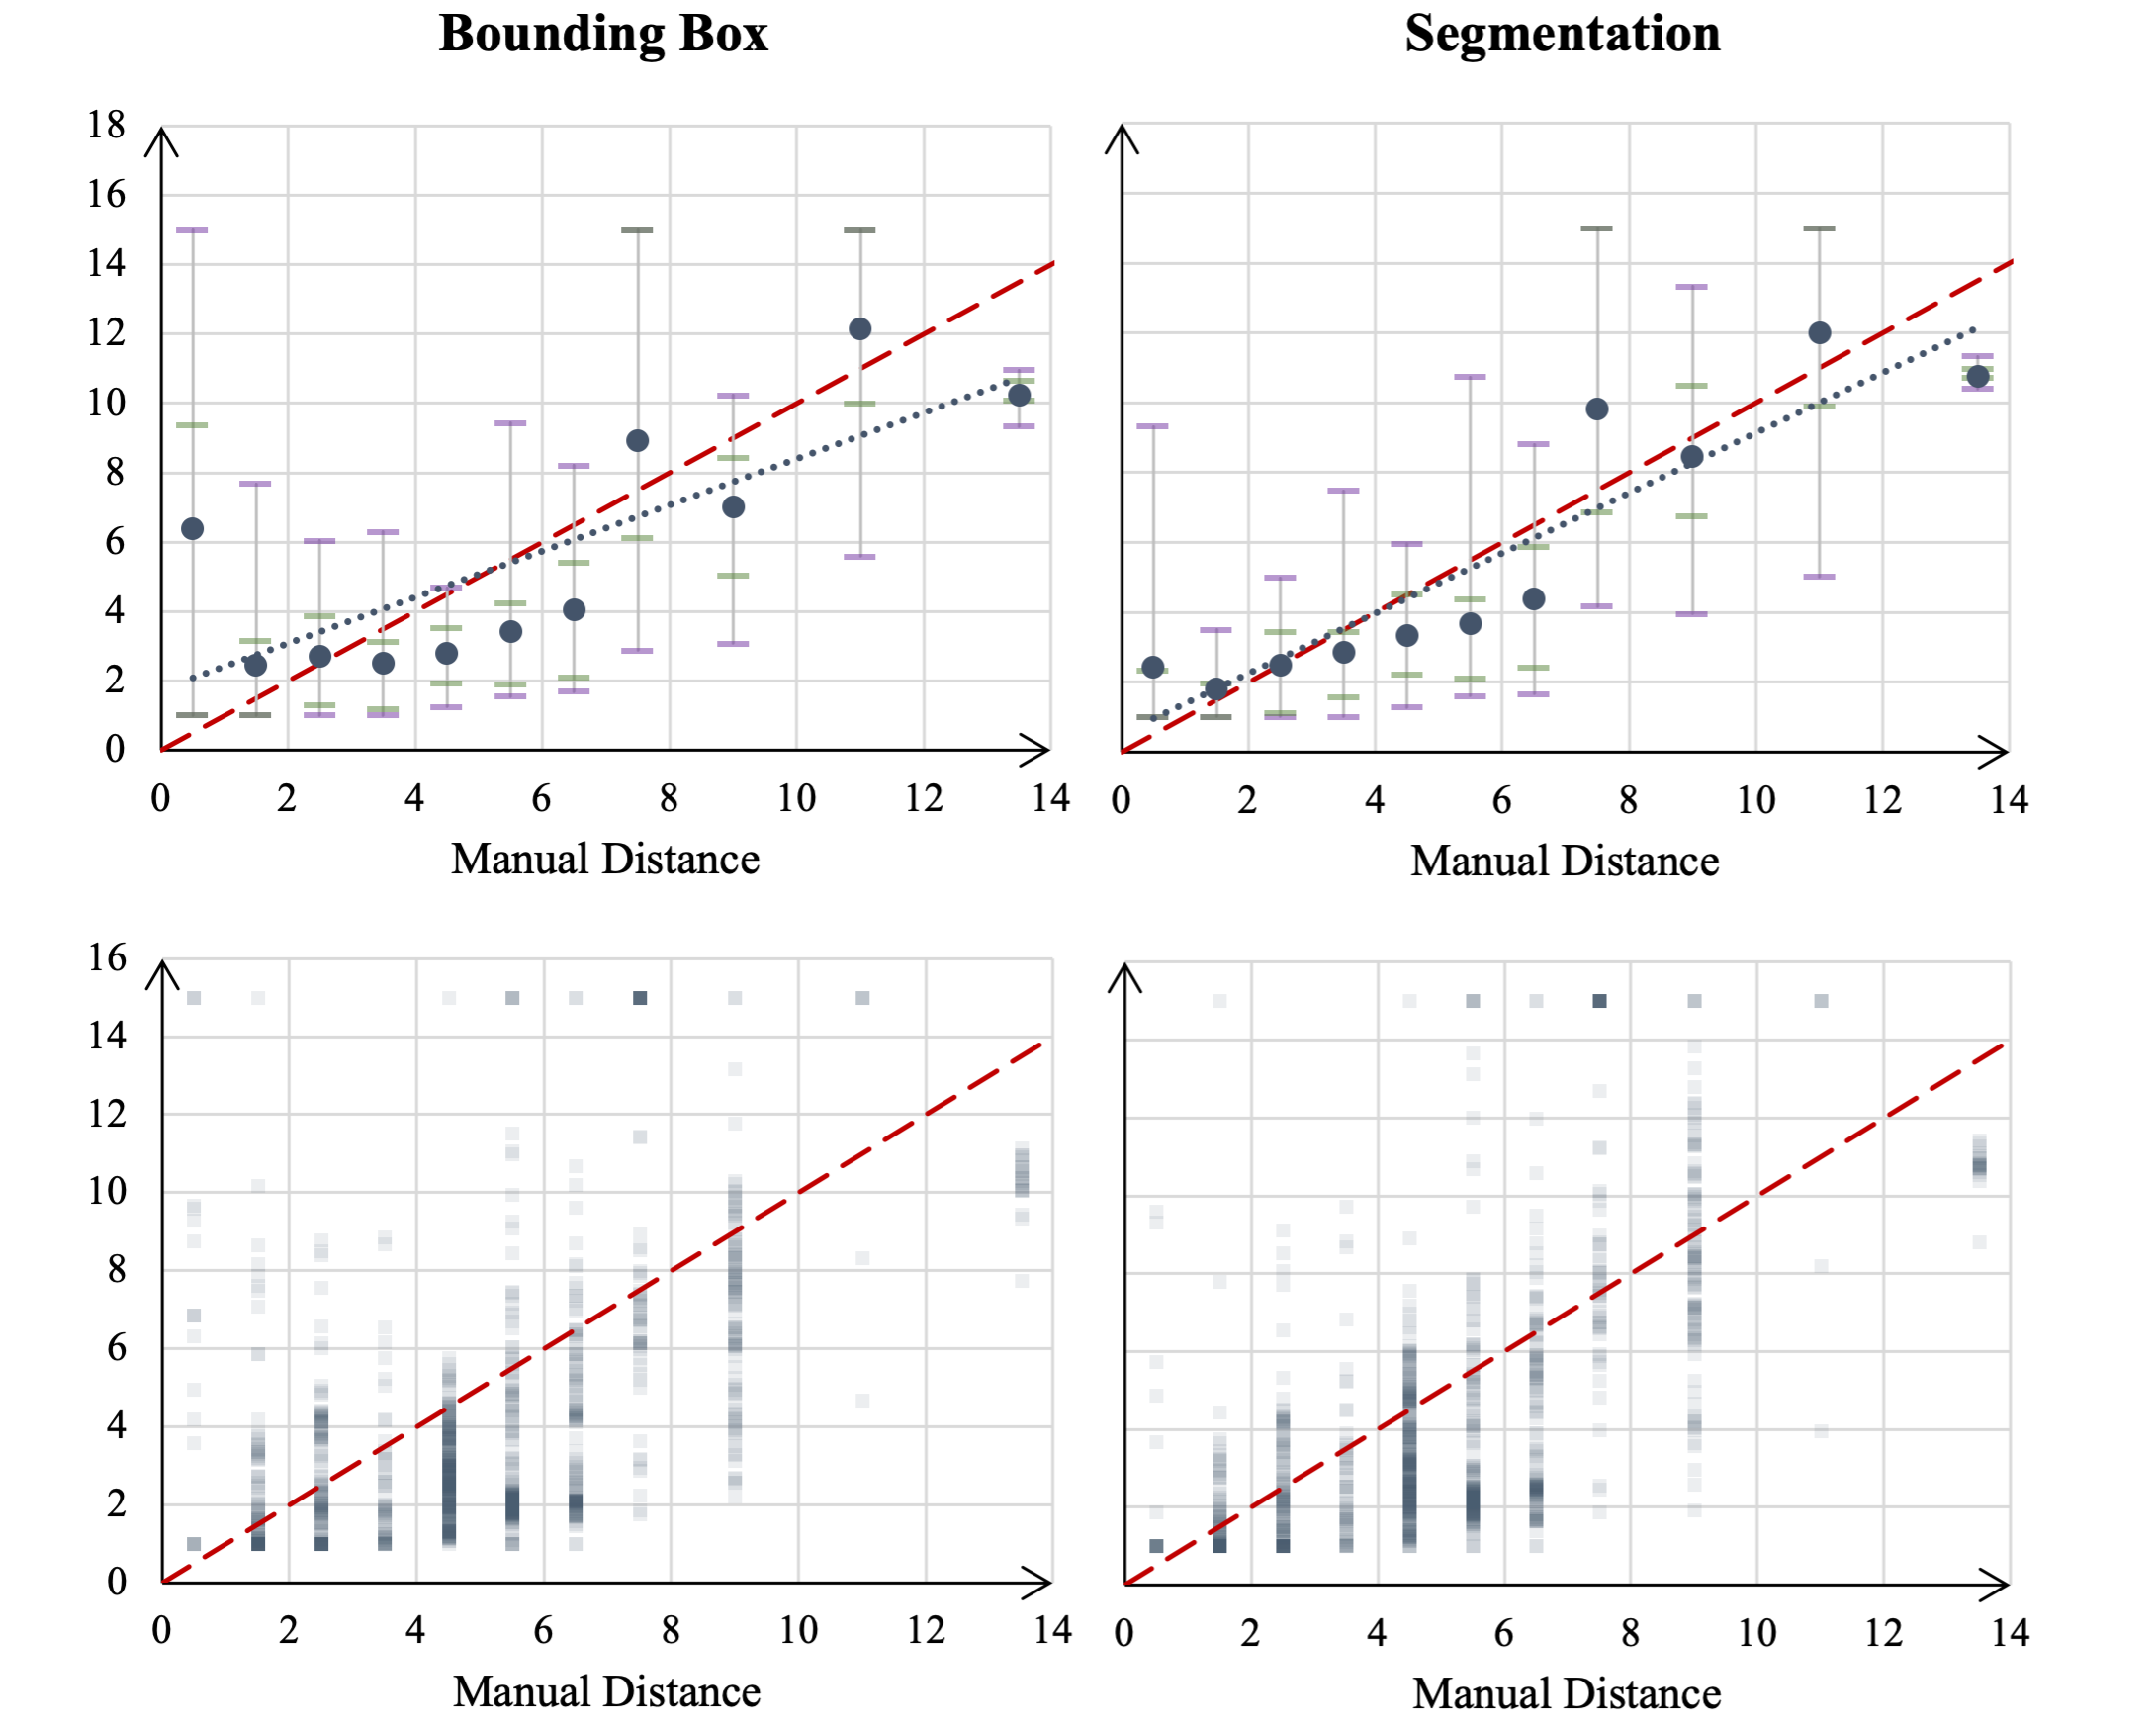
\includegraphics[width=1\textwidth]{body/analysis/assets/distance_graphs/reduced_cal}
    \caption{Graphs showing mean DPT distance estimates (top) and all modelled distance
        estimates (bottom) mapped to thier corresponding manual
        estimates for bounding box (left) and segmentation (right) detection methods using only the
        closest and furthest calibration frames as references. The blue dotted line
        shows the fitted regression line. The red dashed line shows the ideal (i.e., model=manual).
        the error bars show the 25–75 (green) and 5–95 (purple) percentiles. All distances are in
        units of meters.}
    \label{fig:reduced_calibration}
\end{figure}

On inspection of Table~\ref{tab:reduced_calibration_errors} and Figure~\ref{fig:reduced_calibration},
it is evident that this reduced calibration has impacted the results significantly.
The bounding box results give an overall MAE of 2.42 meters and RMSE of 3.13 meters which correspond
to increases of 0.61 meters and 0.47 meters respectively when compared to the results obtained using
all reference frames while the segmentation results give an overall MAE of 2.16 meter and RMSE of
2.83 meters which correspond to increases of 0.46 meters and 0.38 meters respectively.
The spread of the distance estimates have also increased for frames corresponding to all manual
distances.
Moreover, the negative $\Delta_{average}$ values show that this calibration, on average, leads to
underestimation of distances in this dataset

The increase in error of this calibration method is most likely a result of the calibration function
being much more susceptible to any outliers in the DPT estimated depth of the reference frames in
conjunction with any noise/imperfections in the corresponding calibration frame masks.
When many references are used, the impact of sparse outliers are minimised due to calibration
function derivation from predominantly representative data.

More interestingly, the observed shift towards underestimates may be explained by a possible
non-linearity in the relationship between raw DPT generated depth and ground-truth depth.
Specifically, DPT outputs a disparity for each pixel in the processed image.
The calibration frames are used to derive a linear function that maps these raw disparity
values to a calibrated disparity\cite{HAUCKE2022101536} that is equal to inverse distance
(i.e., distance = 1/calibrated disparity).
However, if the true relationship between raw disparity and inverse distance is non-linear,
(e.g., polynomial), a calibration using only the closest and furthest references would result
in a biasing of distance estimates in the mid-distance region.
This effect is visualised in Figure~\ref{fig:disparity_calibration}.

\begin{figure}[H]
    \centering
    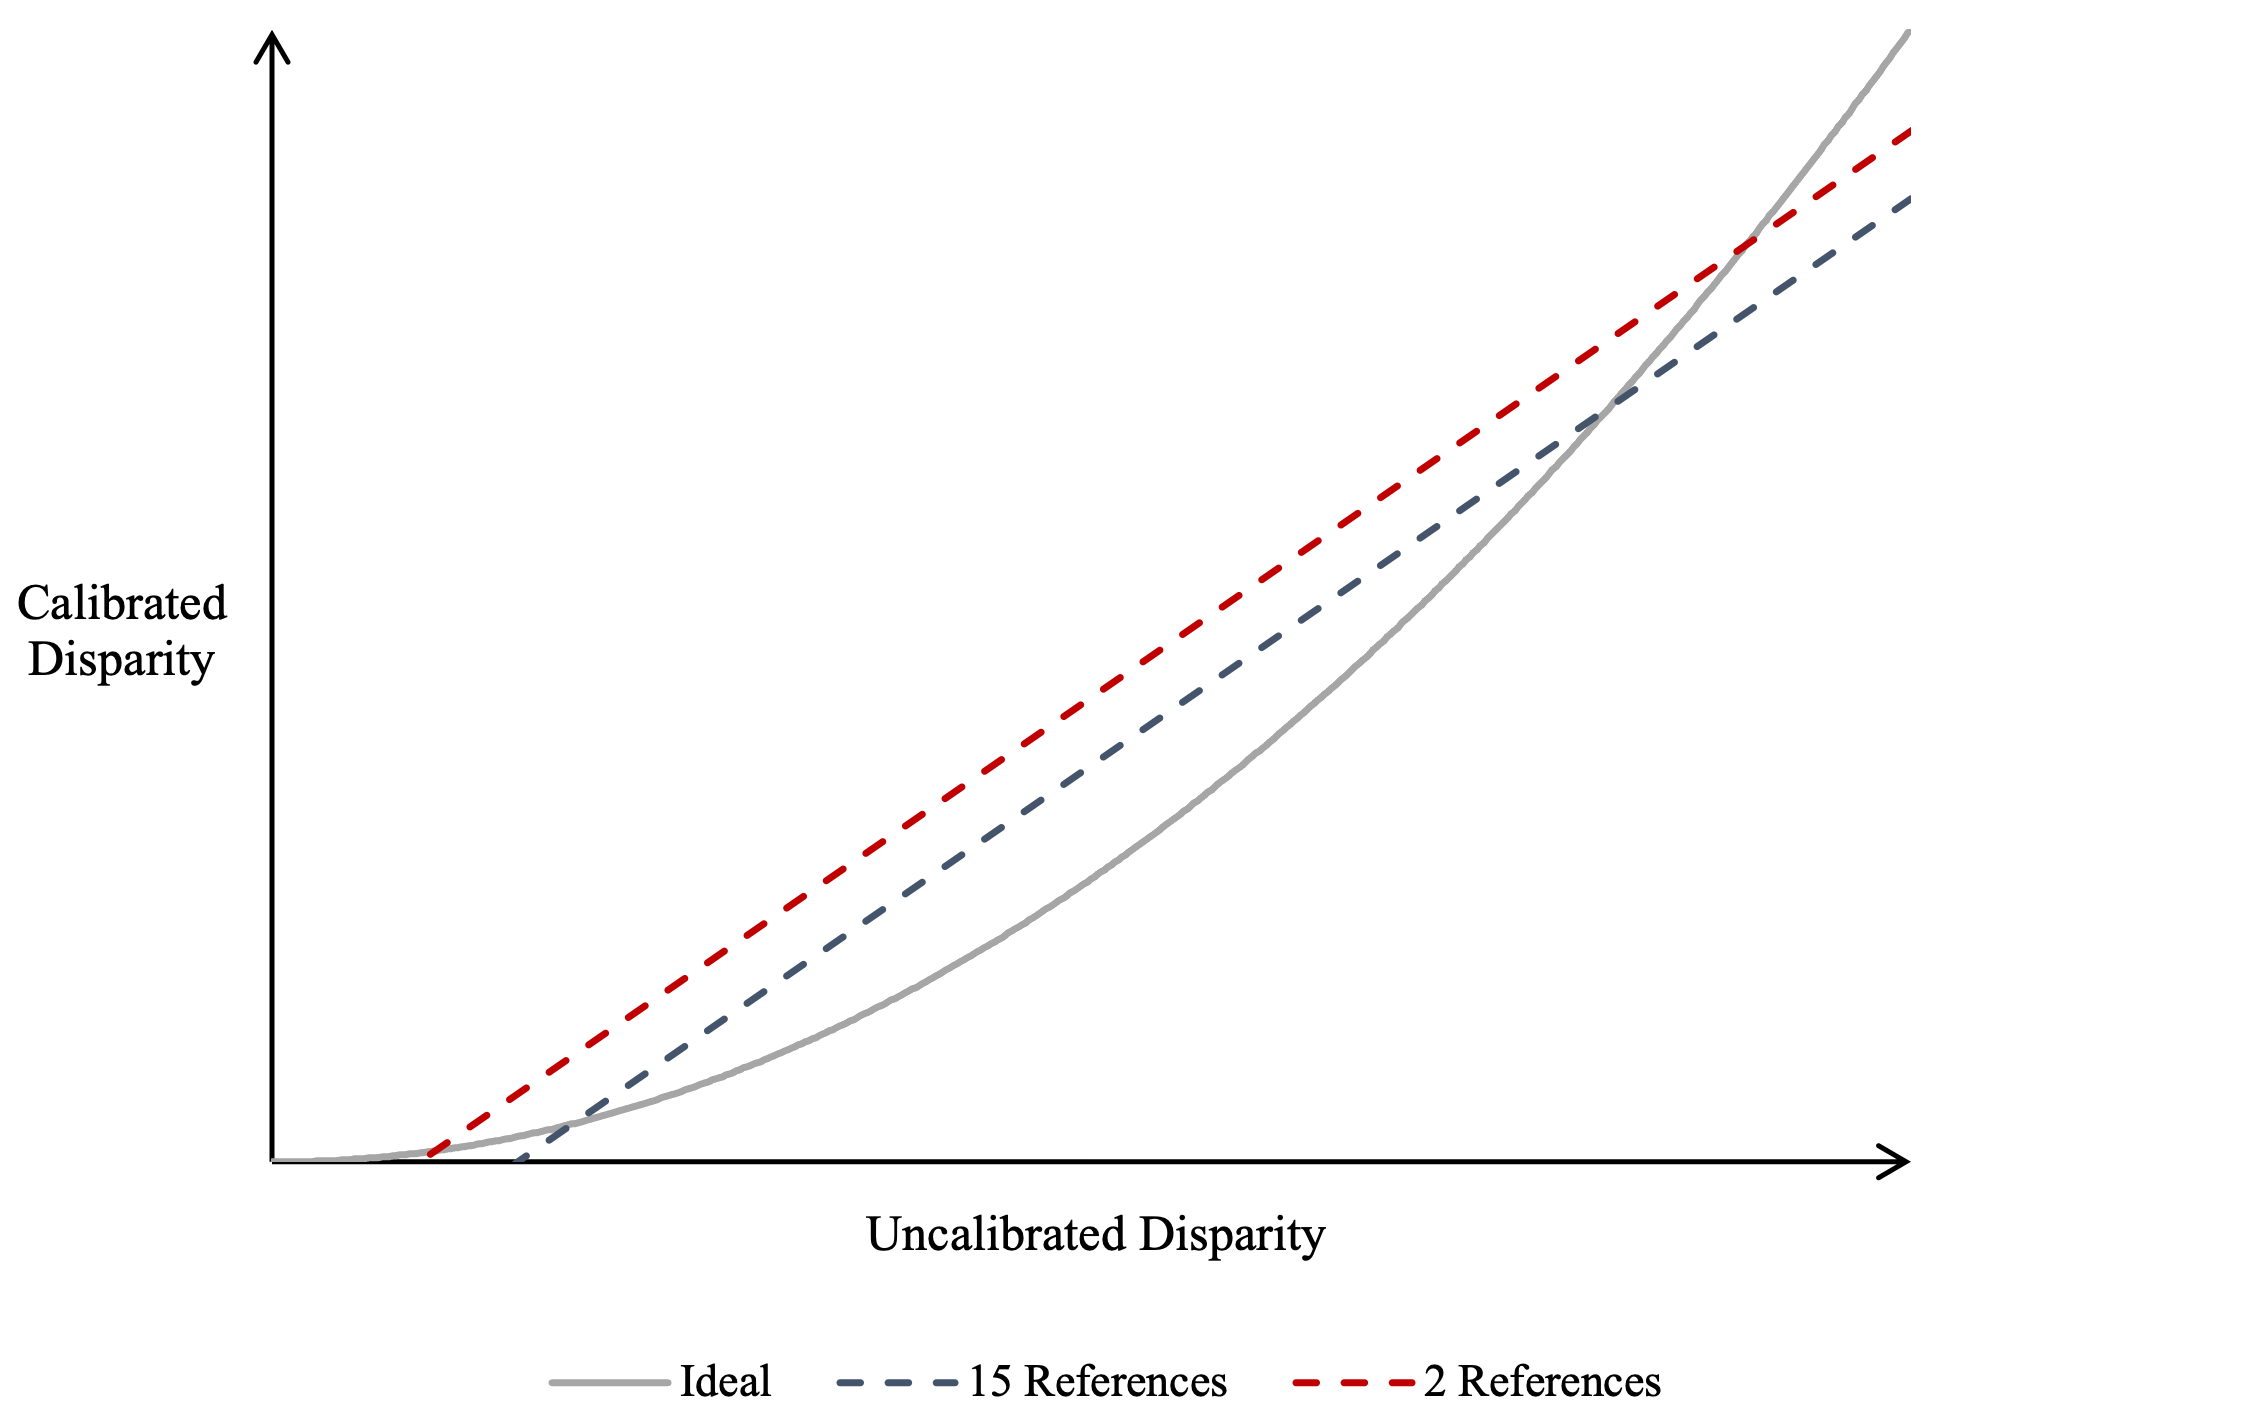
\includegraphics[width=0.7\textwidth]{body/analysis/assets/calibration_effects/disparity_calibration}
    \caption{Simple visualisation showing how the number of reference frames can influence the fitting
        of a calibration function. The grey solid line represents the true mapping of the uncalibrated DPT
        outputted disparity to the calibrated disparity (i.e, 1 / distance). The blue dashed line represents
        a linear disparity mapping fitted using a series of (i.e., fifteen) reference frames while the red
        dashed line represents one fitted using only two (i.e., closest and furthest) reference frames}
    \label{fig:disparity_calibration}
\end{figure}

For example, suppose calibration using all references and calibration using only the closest and furthest
references give the calibration functions
\[
    D_{cal} = 1.5 \cdot D_{raw} - 0.2
    \qquad \mathrm{and} \qquad
    D_{cal} = 1.5 \cdot D_{raw} - 0.05
\]
respectively, where $D_{raw}$ is the raw uncalibrated disparity and $D_{cal}$ is the calibrated disparity
equal to inverse distance.
If a pixel has a raw disparity of $D_{raw}$ = 0.3, applying the 'all references' calibration gives a
calibrated disparity of $D_{cal}$ = 0.25, resulting in an estimated distance of 4 meters while applying
the 'two references' calibration gives a calibrated disparity of $D_{cal}$ = 0.4, resulting in an
estimated distance of 2.5 meters.

This hypothesis is supported when the DPT reference depth maps calibrated using both reference frame
samples are compared.
Figure~\ref{fig:calibrated_maps} shows examples of how the close/far frame calibration results in
a shift in depth towards closer distances.

\begin{figure}[H]
    \centering
    \begin{subfigure}[t]{0.48\textwidth}
        \centering
        \includegraphics[height=0.15\textheight]{body/analysis/assets/calibration_effects/calibrated_maps/all_frames_1}
    \end{subfigure}
    \begin{subfigure}[t]{0.48\textwidth}
        \centering
        \includegraphics[height=0.15\textheight]{body/analysis/assets/calibration_effects/calibrated_maps/two_frames_1}
    \end{subfigure}
    
    \vspace{5mm}

    \begin{subfigure}[t]{0.48\textwidth}
        \centering
        \includegraphics[height=0.15\textheight]{body/analysis/assets/calibration_effects/calibrated_maps/all_frames_2}
    \end{subfigure}
    \begin{subfigure}[t]{0.48\textwidth}
        \centering
        \includegraphics[height=0.15\textheight]{body/analysis/assets/calibration_effects/calibrated_maps/two_frames_2}
    \end{subfigure}

    \caption{Two examples of DPT reference depth maps calibrated using all reference frames
        (left) and reference frames at one and fifteen meters (right). The images on the right
        show a general biasing of depth towards closer distances for pixels in the close to medium
        depth regions.}
    \label{fig:calibrated_maps}
\end{figure}

It is also seen that depth contrast of the far-region pixels is lost is many cases when the
close/far calibration is used (Figure~\ref{fig:far_scale}).
This highlights the importance of using a range of references that correspond to a range of
distances in the far region.
When these are not used in the calibration (in this case), the scale of the calibration function
often fails to capture subtle changes in estimated disparity at far distances.

\begin{figure}[H]
    \centering
    \begin{subfigure}[t]{0.48\textwidth}
        \centering
        \includegraphics[height=0.15\textheight]{body/analysis/assets/calibration_effects/calibrated_maps/all_far}
    \end{subfigure}
    \begin{subfigure}[t]{0.48\textwidth}
        \centering
        \includegraphics[height=0.15\textheight]{body/analysis/assets/calibration_effects/calibrated_maps/two_far}
    \end{subfigure}

    \caption{Example of DPT reference depth maps calibrated using all reference frames (left) and reference
        frames at one and fifteen meters (right). The calibration seen on the rights shows a loss of depth
        contrast in the far-distance region. Here, all pixels corresponding to distances of approximately ten
        meters and over are overestimated to the maximum depth of fifteen meters. The calibration seen on the
        left better captures the depth contrast of the far-region.}
    \label{fig:far_scale}
\end{figure}



%This hypothesis is supported when the average DPT generated distance estimates using all calibration
%frames are compared to those generated using only the closest and furthest calibration frames.
%Figure~\ref{fig:calibration_distance_difference} shows the difference in the distance estimates
%generated by these to calibration methods.
%
%\begin{figure}[H]
%    \centering
%    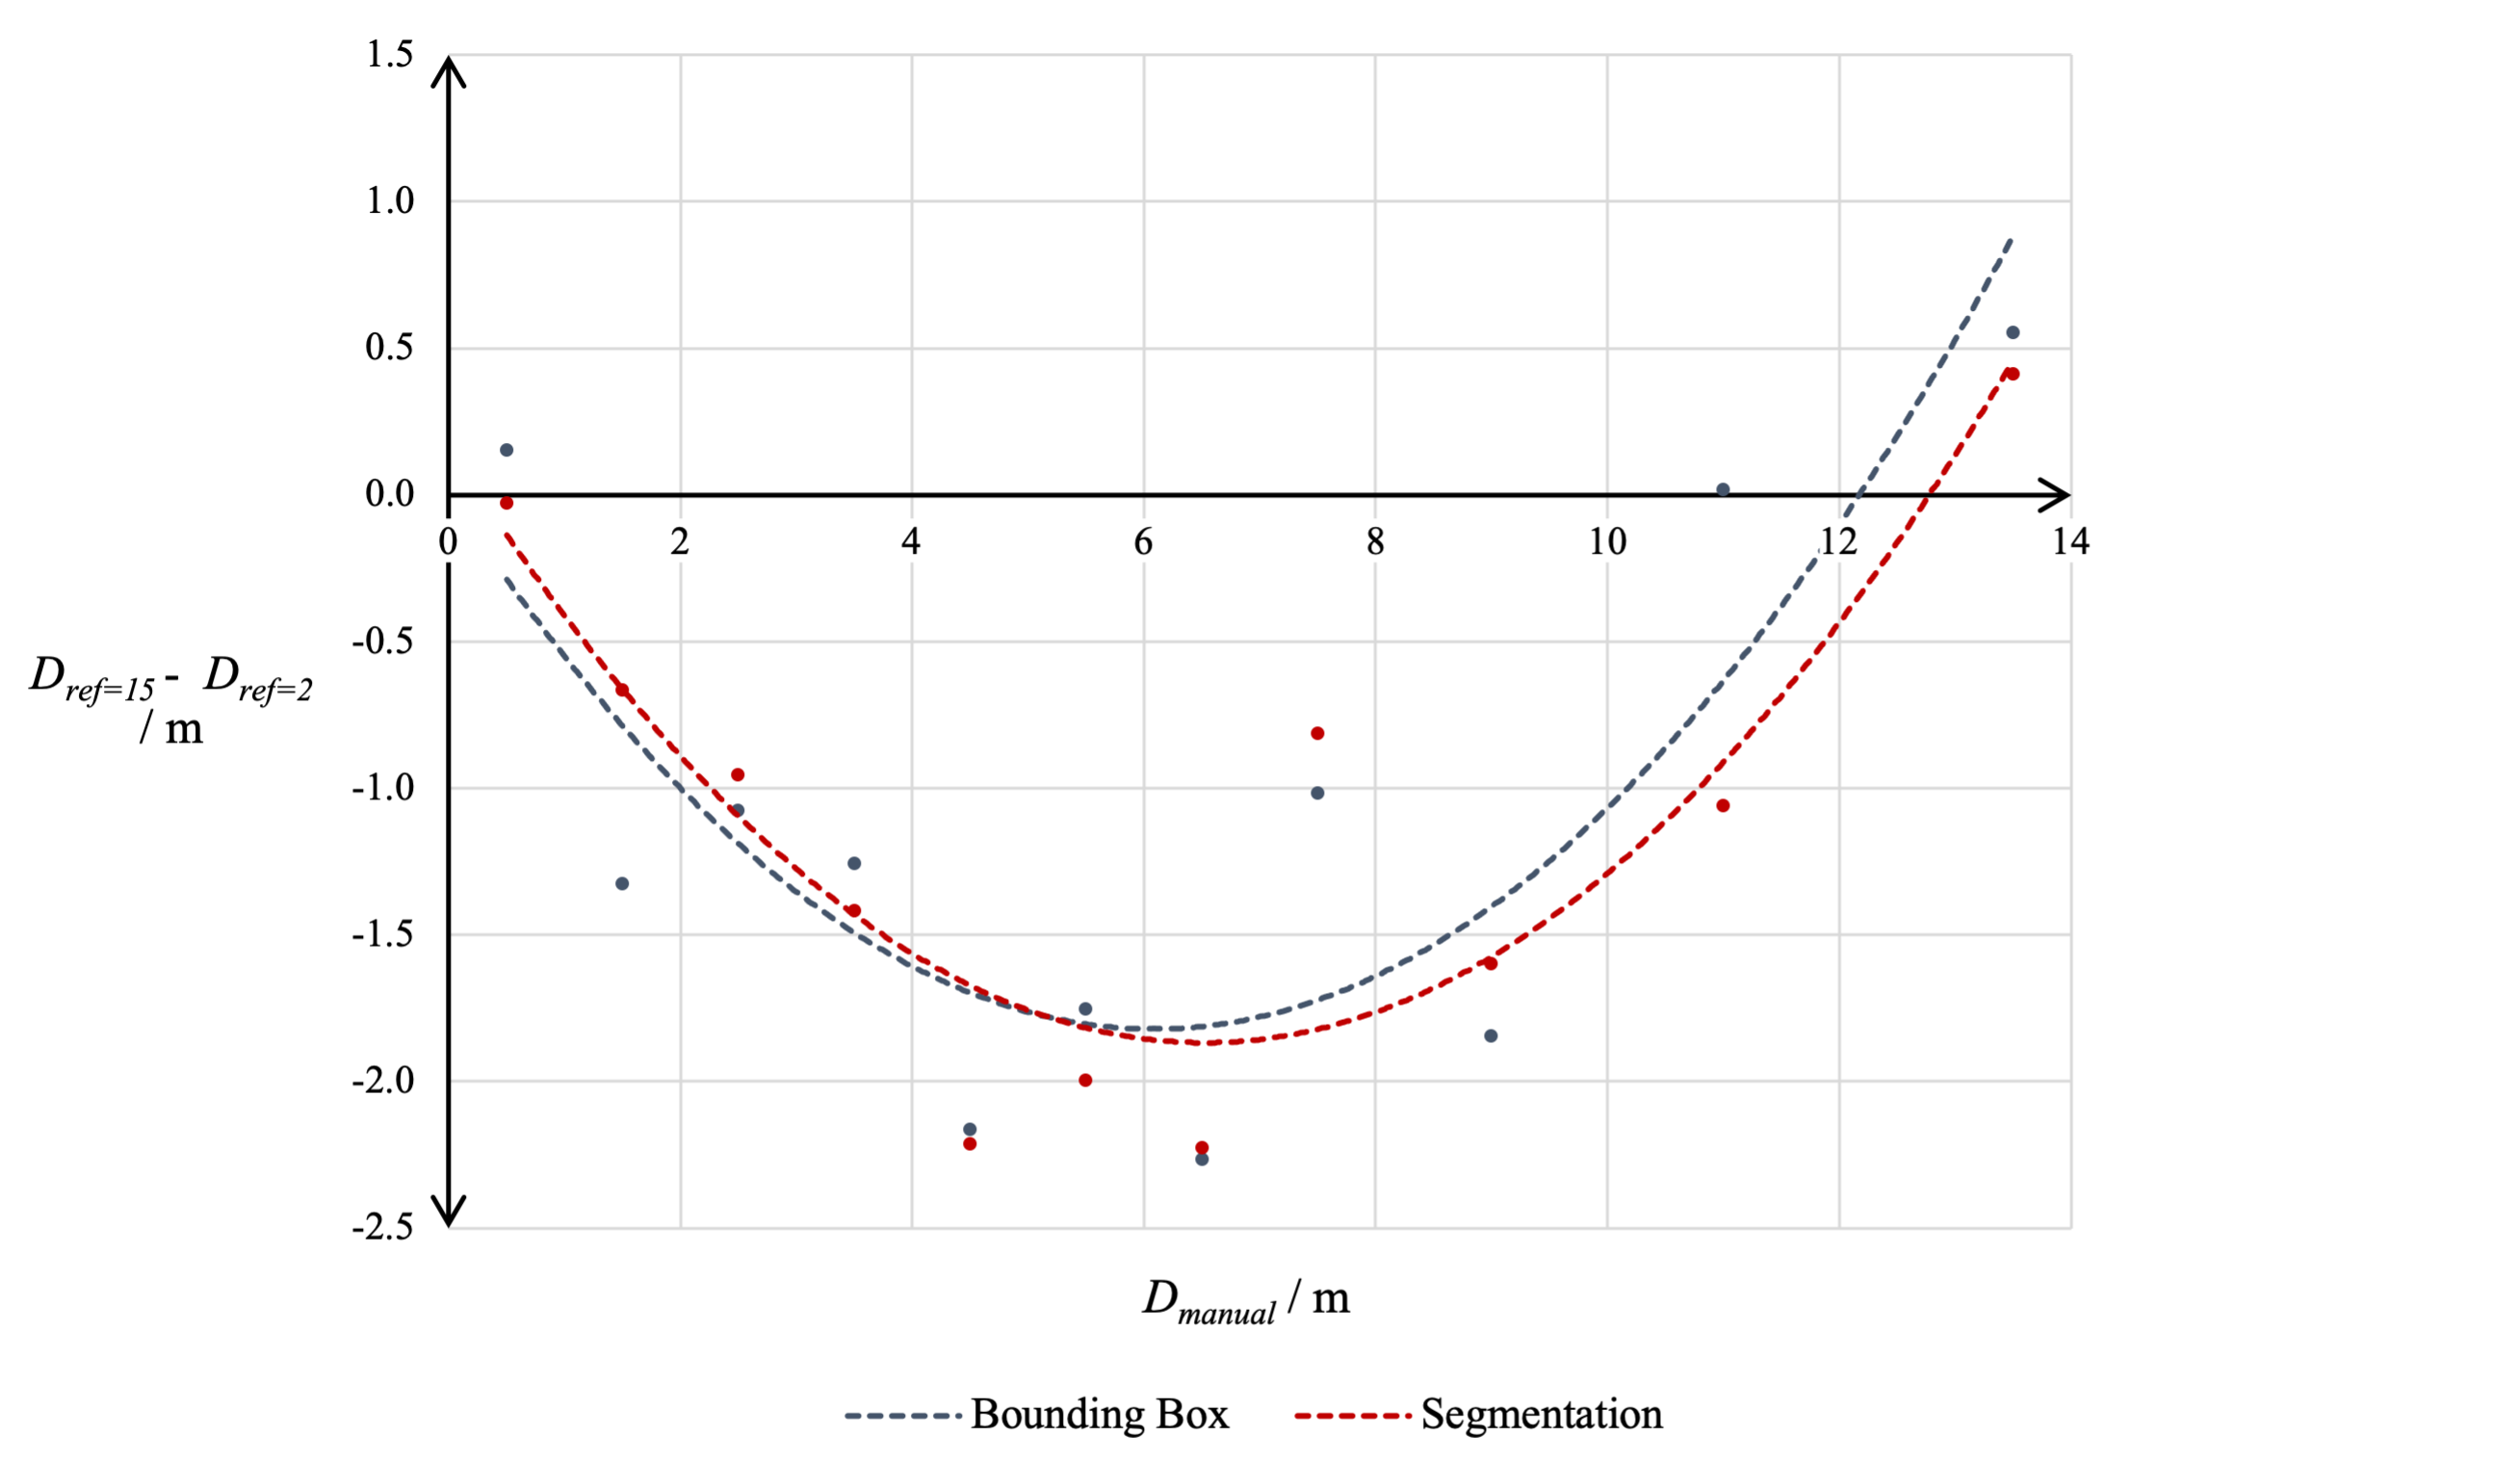
\includegraphics[width=0.85\textwidth]{body/analysis/assets/calibration_effects/calibration_distance_difference}
%    \caption{Graph showing the difference between the average DPT distance estimates calibrated with
%        all reference frames ($D_{ref=15}$) and those calibrated with only the closest and furthest
%        reference frames ($D_{ref=2}$) grouped by corresponding manually estimated distance. Both
%        bounding box and segmentation detection methods are shown.}
%    \label{fig:calibration_distance_difference}
%\end{figure}
%
%These data imply that the true relationship between


\clearpage

\vspace{5mm}
\textbf{Variable Calibration Effects}

To understand the variable calibration results, the mean average error of the distance estimates
with respect to their corresponding manual estimates was calculated for each calibration
of DPT with both bounding box and segmentation detection methods (Figure~\ref{fig:MAE_var_cal}).

\begin{figure}[H]
    \centering
    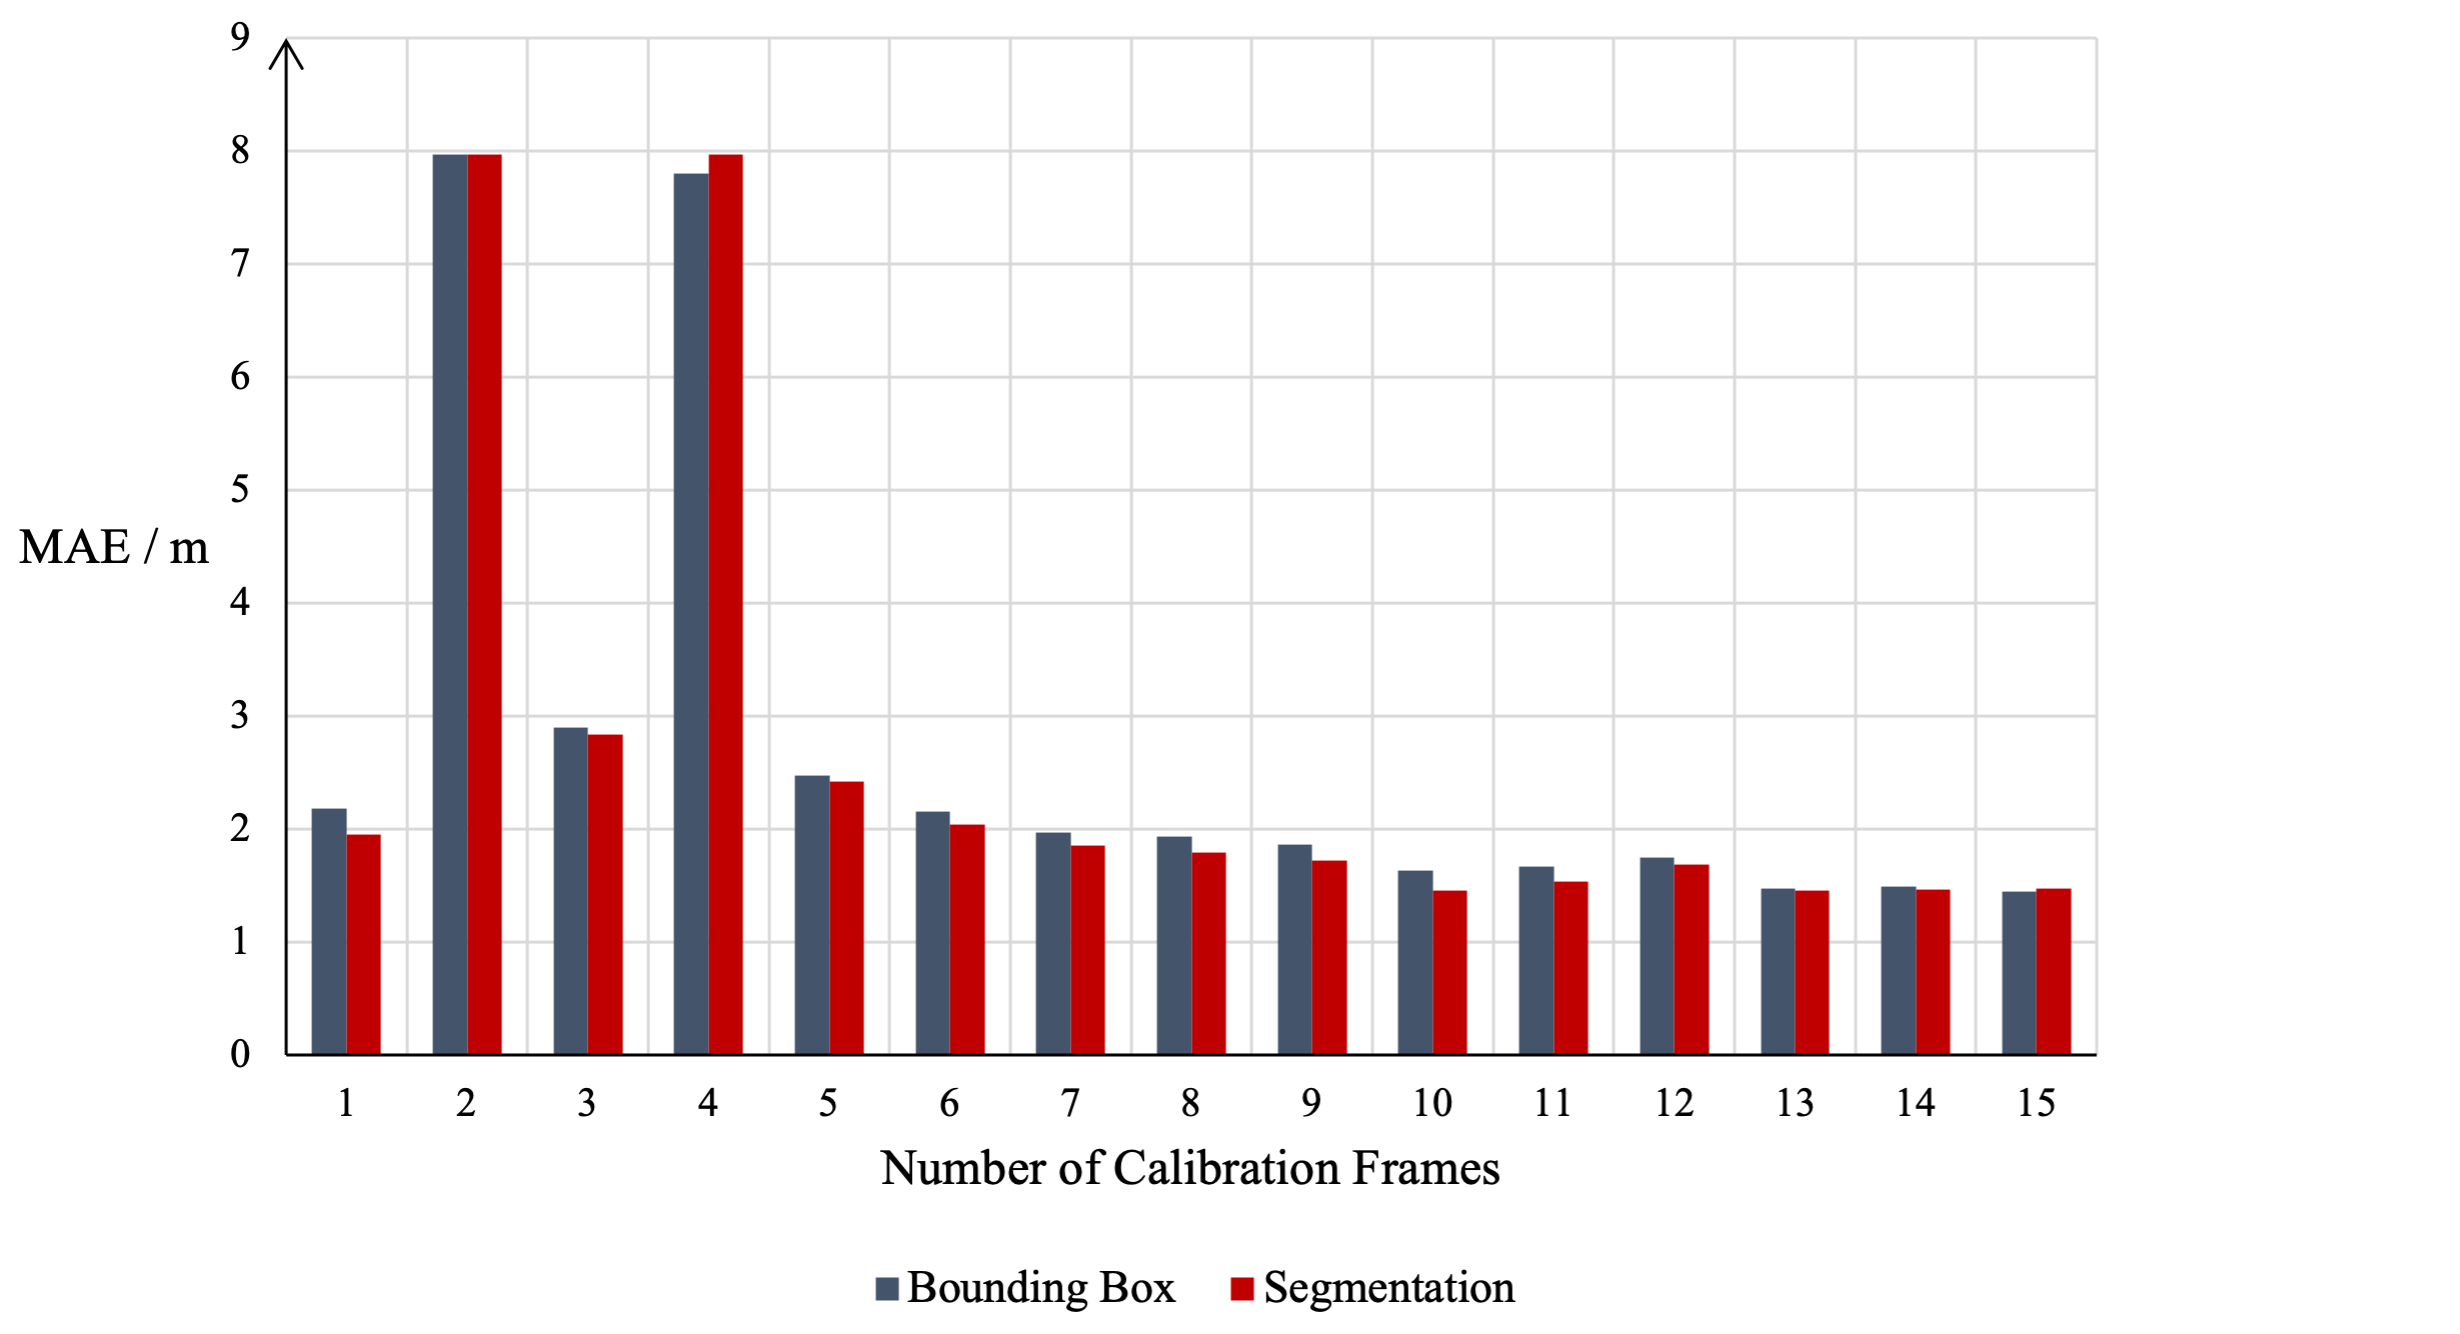
\includegraphics[width=0.7\textwidth]{body/analysis/assets/calibration_effects/MAE_var_cal}
    \caption{Graph showing the mean average error (MAE) of all distance estimates using DPT calibrated
        with a varying number of refrence frames with respect to their corresponding manual distance
        estimate.}
    \label{fig:MAE_var_cal}
\end{figure}

The graph in Figure~\ref{fig:MAE_var_cal} shows minimal difference in error between the corresponding
bounding box and segmentation runs with a general trend towards lower error as the number of reference
frames is incremented, owing to the availability of more points of reference by which the calibration
function is derived.
The error also appears to stabilise onwards from ten references.
This reflects the distribution of distances within the dataset, where the majority of
manual estimates fall into the mid-distance range.
At this particular camera location, the furthest manually estimated distance of any given
observation in the associated detection frames was nine meters, aligning with the observed error
stabilisation from onwards of approximately ten meters, where additional reference frames beyond this
point correspond to distances greater than the maximum observation distance.

To visualise the effect of varying the number of reference frames on calibration, the calibrated
camera location depth maps are shown for each of the runs below (Figure~\ref{fig:variable_calibration}).

\begin{figure}[H]
    \centering
    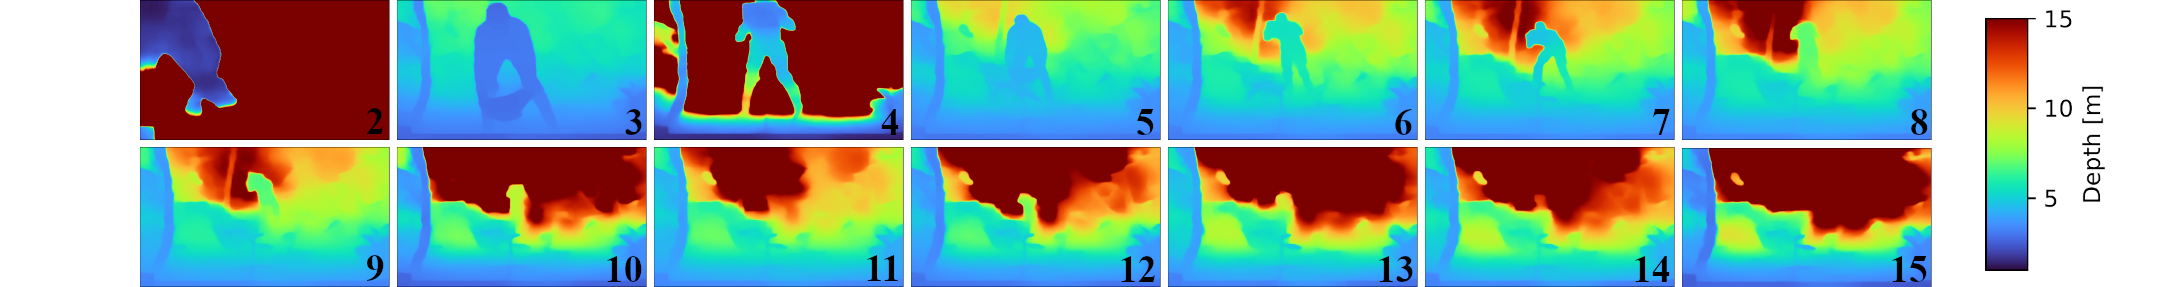
\includegraphics[width=1\textwidth]{body/analysis/assets/calibration_effects/variable_calibation}
    \caption{DPT depth maps of a single camera location generatated using a variable number of
        calibration frames, each labelled with the corresponding number of frames (also the landmark
        distance of the furthest frame) in the bottom-right corner}
    \label{fig:variable_calibration}
\end{figure}

On inspection of Figure~\ref{fig:variable_calibration}, calibrations two and four stand out as having
vastly overestimated background depth.
This shows that, in these cases, the scale of the calibration function is amplified so much as to scale
the disparity of these background pixels to below the maximum depth disparity (i.e., lower than 1/15)
resulting in these pixels being capped at the maximum depth of 15.
This is reflected in Figure~\ref{fig:variable_calibration}, where large spikes are observed in the errors
of the associated distance estimates.

It is not immediately clear why this occurs with just these two calibrations.
Calibration three, despite not capturing the overall depth scale, does not show this effect and
correlates well with the remaining calibration distance estimate errors and depth maps.
A reason may be due to instability of the calibration function when few references are used
resulting from a greater influence from errors in DPT output and calibration frame mask quality;
however, this remains unclear.

It is also worth noting that, in the close distance calibrations (roughly corresponding to the top
rows in Figure~\ref{fig:variable_calibration}), a reference landmark is depicted as a segmented depth
in the depth maps.
This is explained by understanding that the calibrated depth map of a given camera location is
derived from the calibrated reference frame in which that landmark is at the furthest distance form
the camera\cite{HAUCKE2022101536}.
This gives a calibration map where the landmark occupies the smallest number of pixels so to maximise
the background context.
When few references are used, however, the furthest landmark is close and occupies a prominent number
of pixels.

